\documentclass[a4paper, 12pt]{scrartcl}

% !TeX spellcheck = de_AT

\usepackage[utf8]{inputenc}
\usepackage[a4paper, total={7in, 10in}]{geometry}
\usepackage[ngerman]{babel}
\usepackage[T1]{fontenc}
\usepackage{amsmath}
\usepackage{amsfonts}
\usepackage{hyperref}
\usepackage{graphicx}
\usepackage{setspace}
\usepackage[normalem]{ulem}
\usepackage{fancyhdr}
\usepackage{datetime}
\usepackage[style=verbose]{biblatex}
\usepackage{systeme} %for math sys o. equ.
\usepackage{float} %needed to display images
\usepackage{ifthen,xcolor} %somehow needed for tabs
\usepackage{pdfpages} %for importing pdfs
\usepackage{longtable} %for long tables
\usepackage{tabu}%for long tables
\usepackage{footnote}

\newlength{\tabcont} %something with tabs


%systeme config
\sysdelim..
\syslineskipcoeff{1.2}\setlength{\tabskip}{3pt}

\newcommand{\displayauthor}[1]{
	{\small\textit{verfasst von: {#1}}}
}

\newcommand{\blank}[1]{\hspace*{#1}\linebreak[0]}
%user defined commands
\newcommand{\tab}[1]{
	% weils sonst anscheinend keinen tab gibt in latex
	% verwenden:
	% \tab{1} \tab{2}
	% \tab{3} \tab{4}
	% gibt:
	% 1    2
	% 3    4
	\settowidth{\tabcont}{#1}
	\ifthenelse{\lengthtest{\tabcont < .25\linewidth}}
	{\makebox[.25\linewidth][l]{#1}\ignorespaces}
	{\makebox[.5\linewidth][l]{#1}\ignorespaces}
}

\newcommand{\displaycode}[1] {
	% fallst mal versuchst, code mit syntax-highlighting darzustellen:
	% geht anscheinend nicht in makros, da diese code-interpreter
	% angeblich über sich gegenseitig drüberstolpern, habs weder mit
	% 'listings' noch mit 'minted' zum laufen kriegt...
	% is a ziemlicher müll, mach lieber screenshots und füg die ein
	{\fontfamily{qcr}\selectfont #1}
}

\newcommand{\displayownimageg}[3]{
	% wieder gschissen, aber hängt einen Verweis
	% auf den Bildinhaber an
	\displayownimage{#1}{#2}{#3}{0.9}
}

\newcommand{\displayimageg}[2]{
	% oida in latex kamma 'commands' mit untersch. parameteranzahl
	% nicht gleich nennen... ich nenn das jetzt _g für gschissen
	% 0.9 is halt meine standardeinstellung, schaut nicht so deppat
	% aus wie 1, aber ma sieht noch was
	\displayimage{#1}{#2}{#2}{0.9}
}

\newcommand{\displayownimage}[4]{
	\displayimage{#1}{#2}{#2 (Quelle: #3)}{#4}
}

\newcommand{\displayimage}[4]{
	\begin{figure}[H]
	\begin{center}
		\includegraphics[width=#4\textwidth]{#1}
		\caption[#3]{#2} % könnt nützlich werden für das was der schaupp gsagt hat
	\end{center}
	\end{figure}
}

\newcommand{\citebrackets}[1]{
	% wennst iwas zitierst bitte die funktion verwenden. wieder ausm
	% gleichen grund: zentralisieren, wenn iwas net passt, hier ändern
	<<#1>>
}

\newcommand{\makeowntitle}{
	\begin{titlepage}
		\centering
		{\scshape\Large {HTBL Hollabrunn}\\}
		{\scshape\large {Höhere Lehranstalt für Wirtschaftsingenieure}\\}
		{\scshape\normalsize Ausbildungsschwerpunkt Betriebsinformatik\\}
		
		\vspace{4.5cm}
		
		{\huge \textbf{EPIC}}\\
		\vspace{1cm}
		{\LARGE \textbf{Electronic Programmable Intelligent Calculator}}\\
		\vspace{1.5cm}
		%\vfill
		{\Large Michael Friesenhengst, Florian Weinzerl}\\
		\vspace{0.5cm}
		{\Large Betreuer: Ing. Leopold Mayer MBA StR}\\
		\vspace{1.5cm}
		{\large \today}
	\end{titlepage}
}

%add refs
\addbibresource{ref/sachsenschnitzel_references.bib}
\addbibresource{ref/frequem_references.bib}

%\addcontentsline{toc}{section}{Literatur} wemma die Literatur im toc haben wollen, müsst aber noch getweak't werden

\newdateformat{myformat}{\THEDAY{ten }\monthname[\THEMONTH], \THEYEAR}
\pagestyle{fancy}
\fancyhf{}
\rhead{Florian Weinzerl, Michael Friesenhengst}
\lhead{\leftmark}

\DeclareGraphicsExtensions{.pdf,.png,.jpg,.jpeg}
\onehalfspacing

\begin{document}

\makeowntitle
\newpage
{
	\centering
	{\scshape\Large {HTBL Hollabrunn}\\}
	{\scshape\large {Höhere Lehranstalt für Wirtschaftsingenieure}\\}
	{\scshape\normalsize Ausbildungsschwerpunkt Betriebsinformatik\\}
}
\vspace{1.5cm}
\section*{Eidesstattliche Erklärung}
\vspace{0.5cm}
Wir erklären an Eides statt, dass wir die vorliegende Diplomarbeit selbstständig und ohne fremde Hilfe verfasst, andere als die angegebenen Quellen und Hilfsmittel nicht benutzt und die den benutzten Quellen wortwörtlich und inhaltlich entnommenen Stellen als solche erkenntlich gemacht haben.\\
\\
Hollabrunn, am 04.04.2017\\
\vspace{1cm}\\
\textbf{Florian Weinzerl}\\
\\
\rule{8cm}{0.15mm}\\
\\
\textbf{Michael Friesenhengst}\\
\\
\rule{8cm}{0.15mm}
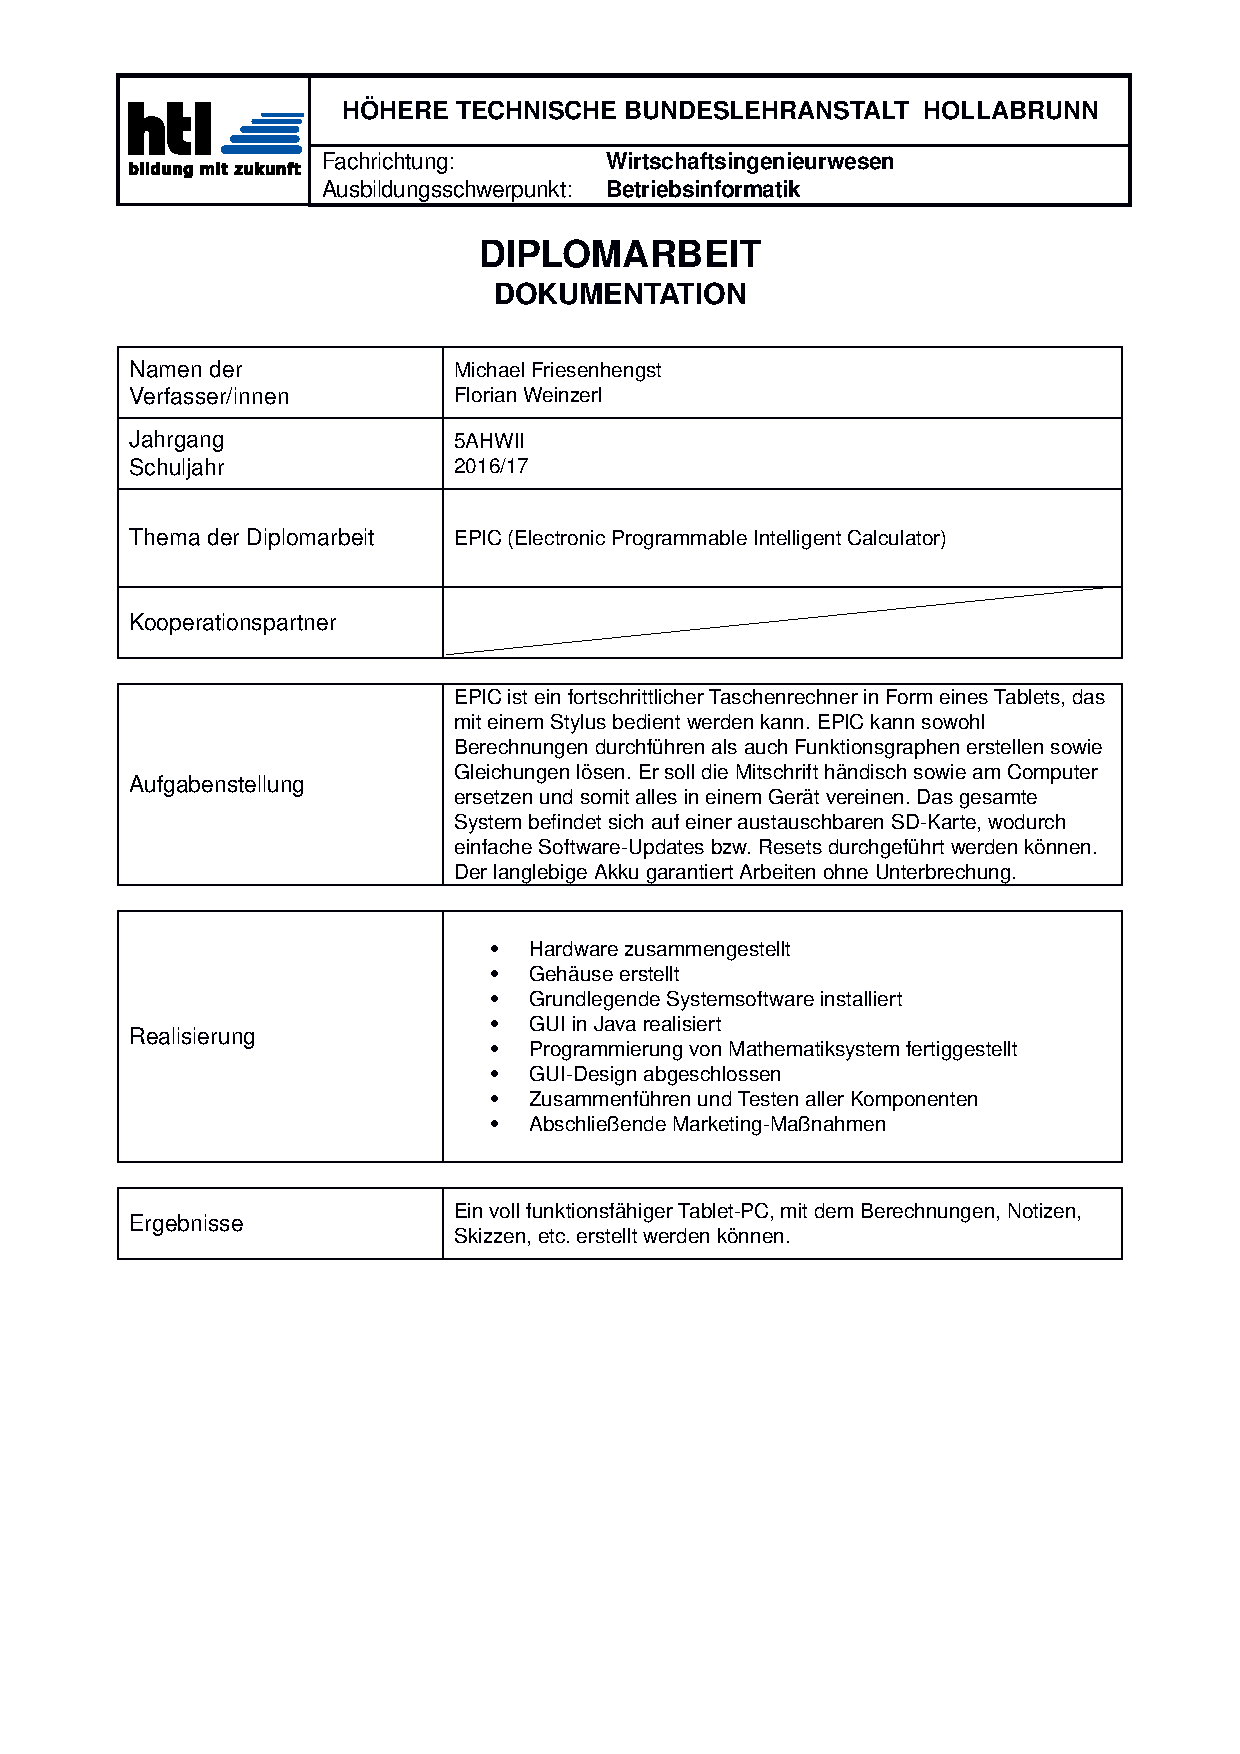
\includepdf[pages={1,2}]{ext/HTL_RDP_Dokumentation_DA_DE_A4.pdf}
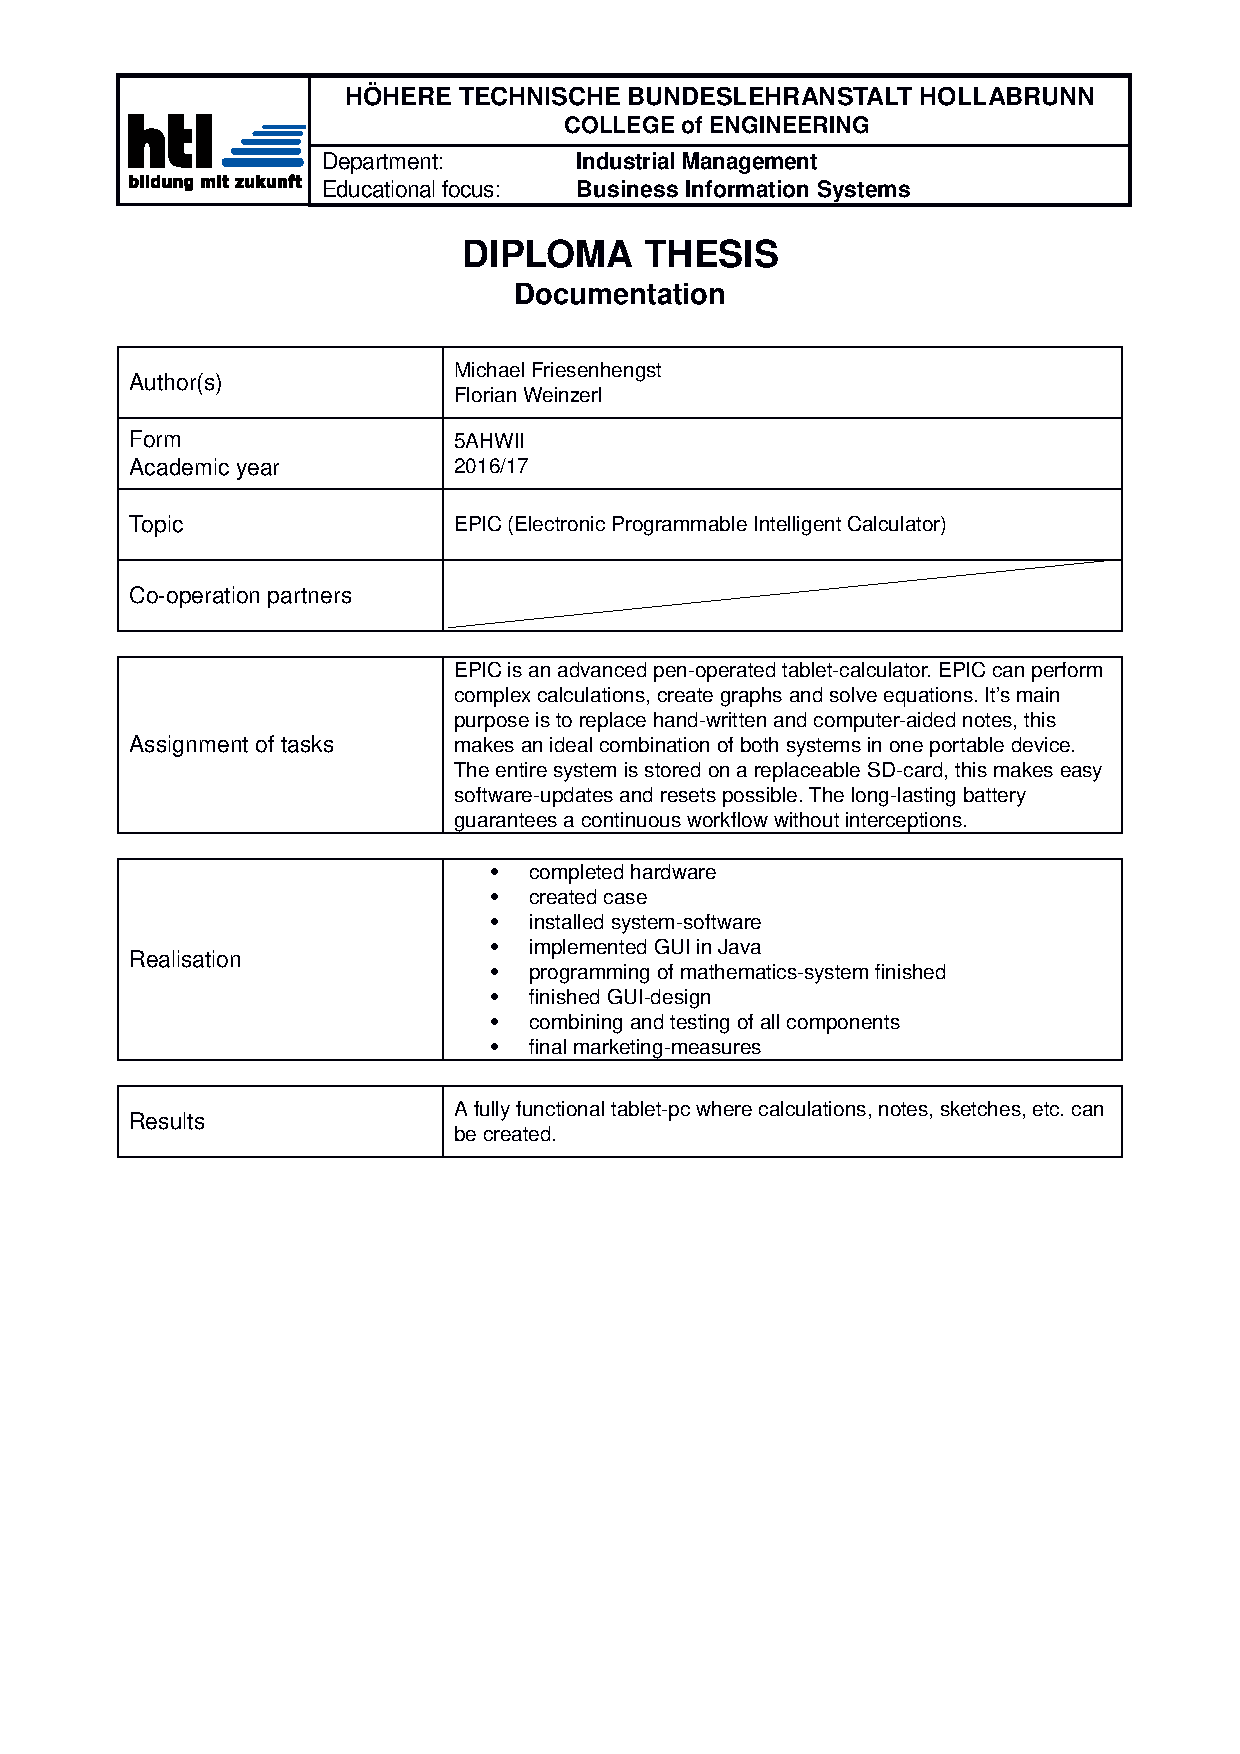
\includepdf[pages={1,2}]{ext/HTL_RDP_Dokumentation_DA_EN_A4.pdf}

\tableofcontents
\newpage

\setcounter{page}{1}
\cfoot{\thepage}

% !TeX spellcheck = de_AT
\section{Einleitung}
Bereits als wir uns erstmalig mit dem Thema, eine Diplomarbeit zu schreiben, auseinandersetzten, war es eindeutig, dass sie nicht bloß sinnhaft und innovativ, sondern darüber hinaus noch eine Herausforderung für uns sein müsste. Ein solches Projekt zu finden, stellte sich als nicht einfach heraus, bis schlussendlich ein Problem aus dem Schulunterricht auftrat. Das Wort ''Problem'' soll hier weniger für eine Störung stehen, wie es in unserem Sprachgebrauch oft verwendet wird, viel mehr ist damit ''Problemstellung'' gemeint.\\\\
Unsere jeweiligen Schulkarrieren wurden denkbar auf Papier begonnen und allmählich würde ein Fach nach dem anderen auf digitale Mitschrift durch Laptop oder ähnliches umsteigen. Heute und vermutlich noch sehr lange Zeit besteht dies aus einer Mischform: Wer bestmöglich im Unterricht dabei sein will, sollte Texte notieren, möglicherweise auf Dateien aus dem Internet zugreifen, Freihandzeichnungen von der Tafel auf die eigenen Zettel übertragen und die Lösung des einen oder anderen Gleichungssystems nachvollziehbar dokumentieren können und wenn möglich alles so speichern respektive hinterlegen, dass es einfach wieder auffindbar ist. Unserer Meinung nach sind das zwar Aufgaben, die bewältigbar sind, aber wenn es möglich wäre all diese Aufgabenbereiche in ein Gerät zu kombinieren, das demnach im Unterricht, in Vorlesungen, aber auch in manchen technischen Berufen genutzt werden kann, so ist das Ergebnis nicht nur eine Entlastung, sondern schließt womöglich auch eine Marktlücke.\\\\
Und genau das haben wir uns zur Aufgabe gemacht. Wenn Sie als Leser eine kurze Werbung erlauben, hier ist die fertig verfasste Aufgabenstellung an uns selbst während der Arbeit:\\\\
\textit{EPIC ist ein fortschrittlicher Taschenrechner in Form eines Tablets, das mit einem Stylus bedient werden kann. EPIC kann sowohl Berechnungen durchführen als auch Funktionsgraphen erstellen sowie Gleichungen lösen. Er soll die Mitschrift händisch sowie am Computer ersetzen und somit alles in einem Gerät vereinen. Das gesamte System befindet sich auf einer austauschbaren SD-Karte, wodurch einfache Software-Updates bzw. Resets durchgeführt werden können. Der langlebige Akku garantiert Arbeiten ohne Unterbrechung.}\\\\
Dinge, die uns außerdem wichtig sind, umfassen unter anderem Modularität und das korrekte Marketing, was wir uns anschließend auch zur Aufgabe machten.

\subsection{Gedanken zur Umsetzung}
%Wollma bei der Umsetzung dazu schreiben, wer was gmacht hat? oder iwo anders?
Nun stellt sich also die Frage: Wie wollen wir all das bewerkstelligen? Die hardwaretechnische Einschränkung auf ein Tablet erleichtert die Entscheidung schon um Einiges. Im Hinblick darauf fassten wir den Entschluss, einen kleinen \textit{single-board-computer} zu verwenden, welcher sowohl software- als auch hardwaretechnisch in der Lage ist, unsere Software zu unterstützen. Hier hat sich ein \textit{Raspberry Pi} angeboten, da es für diesen im \textit{World Wide Web} eine große \textit{Community} gibt, die bei Auftreten von Problemen helfen kann. Weiters bietet der Raspberry Pi den wahrscheinlich größten \textit{Support} von \textit{Hardware-Treibern} im gesamten single-board-computer Marktsegment.\\
\\
Um auf dem Tablet vernünftig arbeiten zu können, machten wir uns Gedanken über den zu verwendenden Display, wie groß dieser sein sollte und welche Auflösung dieser haben musste. Nach mehreren Design-Iterationen einigten wir uns auf einen 7'-Display mit \textit{resisitiver Touch-Eingabe}, um mit einem Stift arbeiten zu können. Wir empfanden es als äußerst wichtig, einen \textit{Stylus} verwenden zu können, dieser erleichtert nämlich die Eingabe, vor allem bei Schreibaufgaben, gegenüber einem Finger, welcher bei klassischen Tablets verwendet wird.\\
\\
Um unsere Recheneinheit sowie den Display ein- und ausschalten zu können musste ein \textit{Mikrocontroller} her, welcher im \textit{Standby-Modus} einen minimalen Energieaufwand aufweist um eine lange Akku-Laufzeit zu garantieren. Hier bot sich ein \textit{Arduino Pro Mini} an, da dieser ohne Überflüssigen Overhead, der lediglich die Akku-Laufzeit verkürzen würde, auskommt. Ein weiteres wichtiges Kriterium für uns war auch, dass sich der Mikrocontroller mit bekannten Mitteln programmieren lässt. Da man den Arduino mit der Programmiersprache \textit{C} programmieren kann, wurde dieser gewählt.\\
\\
Der Endnutzer möchte diese Hardware natürlich nicht sehen, sondern lediglich von seiner Funktion profitieren, deshalb wird ein Gehäuse benötigt, welches groß genug ist um allen Hardware-Komponenten Platz zu bieten, klein genug ist, um es ohne Probleme transportieren zu können und robust genug ist, damit man ohne besonders Acht zu geben darauf arbeiten kann. Da es so ein Gehäuse nicht vorgefertigt zu kaufen gibt, mussten wir dieses selbst designen und produzieren. Bei diesem Prozess war es wichtig, \textit{CAD}-Kenntnisse zu besitzen, diese anzuwenden und anschließend das Werkstück zu fertigen. Da es sich bei der Hardware um einen Prototypen handelt musste eine Methode her, das Gehäuse billig und ohne großen Aufwand herzustellen. Hier bot sich \textit{3D-Drucken} an, da es sämtliche Kriterien erfüllt.\\

%Software
\ \\
Bezüglich der Software konnte wohl nicht viel aus fremden Komponenten verwendet werden, vor allem, da das dem Sinn dieser Arbeit widersprechen würde. Wir waren also selbst dafür zuständig und das bedeutete, sowohl die Benutzer-Oberfläche als auch die Schreib- und Mathematik-Einheit waren so zu realisieren, dass auch nach Abschluss und Veröffentlichung Entwickler auf dem Code aufbauen können. Das hat zusätzlich den taktischen Vorteil, dass Benutzer bei Bedarf auch schnell eigene Funktionen hinzufügen und diese dann für Andere zugänglich machen können. Diese Funktionalitäten sind zwar von den üblichen Taschenrechnern bekannt, allerdings nicht in einer plattformunabhängigen Sprache, die darüber hinaus objektorientiertes Programmieren ermöglicht, wie Java.
%eigentlich iss ja net ganz teil der diplomarbeit, aber schau ma obs ihm auffallt?:
Potenzielle Kunden hätten also den Vorteil, dass sie selbst darüber verfügen können, welche Software-Pakete sie neben den Grundfunktionalitäten integriert haben möchten. Das bezieht sich auch darauf, dass sie vom Programmiertalent Anderer profitieren können, falls eine eher ausgefallene oder fachspezifische Funktion per Softwaremodul von einer Privatperson ins Internet hochgeladen wurde.\\
\\
Betreffend der Oberfläche ist sicher ein Menü am oberen Fensterrand sinnvoll. Dieses sollte Menüpunkte in Kategorien einteilen, und dem Benutzer die häufigst verwendeten Funktionen schnell zugreifbar machen. Dies sind möglicherweise keine überraschenden Festlegungen, aber zu irgendeinem Zeitpunkt müssen Design-Entscheidungen getroffen werden. Außerdem weist nicht jedes Menü diese Flexibilität auf, ob sie sich bewährt wird man sehen, und diese Eigenschaft kann eventuell noch nachjustiert werden.
Darüber, was die Mathematik-Einheit zu bieten haben sollte, lässt sich wohl kaum streiten. Die Vorgaben dafür beschränken sich, bis auf dass sie funktionstüchtig sein soll, auf Null.\\
\\
Dafür ist das Marketing eine äußerst interessante, um nicht zu sagen eine schwungvolle Angelegenheit. Dabei wollen wir uns in unsere potenziellen Kunden hineinversetzen und erforschen, warum sie unser Produkt kaufen, wie der Entscheidungsprozess stattfindet und in wie fern wir uns das für unseren Imageaufbau und Vermarktung des Produkts zu Nutzen machen können.\\
\\
Um die Arbeitseffizienz zu erhöhen und gleichzeitig die Wissensbereiche der Beteiligten optimal auszuschöpfen, wurde eine Aufteilung der Arbeit getroffen. Herr Michael Friesenhengst übernahm dabei die Erstellung der Hardware und das Ausprogrammieren der \textit{GUI}. Herr Florian Weinzerl war für das Mathematik-Paket und dessen Implementation in die GUI zuständig. Das Marketing haben sich beide zur Aufgabe gemacht, da dort die besten Ergebnisse in der Diskussion zustande kommen.
\section{Bedienungsanleitung}\displayauthor{Michael Friesenhengst}
\subsection{Hardware-Bedienung}

\subsubsection{Powerbutton}

Der Powerbutton wird verwendet, um EPIC einzuschalten, den Standbyzustand zu beenden, ihn zu starten oder um EPIC auszuschalten. Beim Versetzen in den Ruhezustand wird der Bildschirm ausgeschaltet, was Strom spart und das Berühren unbeabsichtigter Funktionen verhindert.\\
\\
Die Standbytaste befindet sich seitlich rechts.


\paragraph{EPIC einschalten:}
Halten Sie den Powerbutton für mind. 3 Sekunden gedrückt. Nach anschließendem Loslassen wird EPIC eingeschaltet.

\paragraph{EPIC ausschalten:}
Halten Sie den Powerbutton für mind. 3 Sekunden gedrückt. Nach anschließendem Loslassen wird EPIC heruntergefahren und ausgeschalten.

\paragraph{Standbymodus starten:}
Drücken Sie kurz auf den Powerbutton und lassen Sie diesen umgehend wieder los. Ist der Bildschirm von EPIC abgeschaltet, so ist der Standbymodus aktiv.

\paragraph{Standbymodus beenden:}
Drücken Sie kurz auf den Powerbutton und lassen Sie diesen umgehend wieder los. Das Gerät ist nun wieder einsatzfähig.

\subsubsection{Mikro-USB-Anschluss}

Verbinden sie ein passendes USB-Kabel mit dem Mikro-USB-Anschluss um EPIC aufzuladen. 

\subsubsection{USB-Anschluss}

Der USB-Anschluss kann wie ein regulärer USB-Port eines PCs genutzt werden. Es können unter anderem USB-Memory-Sticks, Tastaturen oder Mäuse verbunden und genutzt werden.

\subsubsection{Touchscreen}

Der Touchscreen wird mithilfe eines Stiftes bedient, dieser sollte eine Plastik- oder Nylonspitze haben, um problemlos auf dem Touchscreen zu gleiten. Um gute Ergebnisse zu erzielen, wird empfohlen ca. 1,5x so fest aufzudrücken, wie man es mit einem Kugelschreiber gewöhnt ist. 

\subsection{Software-Bedienung}

\subsubsection{Spritepanel}
Das Spritepanel ist der große weiße Bereich in der Mitte des Fensters. Darauf werden alle Aktionen durchgeführt, es werden Berechnungen getätigt, Skizzen angelegt oder Notizen verfasst. Einzelne Objekte, welche auf dem Spritepanel angezeigt werden können wie Text oder Zeichnungen, werden als Sprites bezeichnet.

\subsubsection{Verwenden der On-Screen-Tastatur}

Die On-Screen-Tastatur ist nach dem Hochfahren standardmäßig maximiert angezeigt. Um die Tastatur zu minimieren, wird auf den standardmäßig rechts unten am Bildschirm angezeigten Keyboard-Icon geklickt, dieser wird ebenfalls verwendet, um die Tastatur zu maximieren. Der Icon und die Tastatur können durch Halten und Bewegen des Stiftes am Bildschirm verschoben werden.


\subsubsection{Menubar}

Die Menubar ist der Menübereich über dem Spritepanel. Er ist zur Konfiguration und zum Starten verschiedener Operationen gedacht. Um eine Operation zu starten oder eine Einstellung zu treffen, wird auf die jeweiligen Buttons, die nach Kategorien aufgelistet sind, geklickt. In manchen Fällen, sind zu viele Operationen (Menuitems) innerhalb einer Kategorie verfügbar, in diesem Fall wird unten ein Button zur Erweiterung des Menüs angezeigt. Wird auf diesen Button geklickt, so öffnet sich ein neues Fenster, auf dem die zusätzlichen Auswahlmöglichkeiten angezeigt werden. Diese können wie gewohnt mittels Klick auf den Touchscreen verwendet werden.

\subsubsection{Modes}

Verschiedene Modes werden auf der Menubar ausgewählt.

\paragraph{Draw Mode:}
Im Draw-Mode können Zeichnungen, Skizzen und handschriftliche Notizen angelegt werden. Wählen Sie dazu den Draw Mode in der Menubar aus, anschließend können durch Streichen des Stiftes über den Bildschirm auf dem Spritepanel Zeichnungen angelegt werden. Wird der Stift vom Spritepanel abgesetzt, so wird beim nächsten Streichen ein neues Sprite angelegt, mit dem unabhängig vom alten gearbeitet werden kann.

\paragraph{Text Mode:}

Im Text-Mode können mithilfe der On-Screen Tastatur Texte verfasst werden. Nach dem Auswählen des Text-Modes in der Menubar kann auf eine beliebige Stelle im Spritepanel geklickt werden. An der gewählten Stelle erscheint ein blauer Cursor, mithilfe der Tastatur kann nun ein Text verfasst werden.\\
\\
Im Text-Mode können mithilfe des Cursors auch mehrere Buchstaben ausgewählt werden um diese beispielsweise zu ersetzten oder zu löschen. Dazu können innerhalb eines Text-Sprites Textstellen mit dem Stift markiert werden, wobei ausgewählte Buchstaben blau hinterlegt werden. Markierte Buchstaben können durch Schreiben auf der Tastatur ersetzt bzw. mithilfe der Backspace-Taste gelöscht werden.

\paragraph{Math Mode:}

Im Math-Mode können mithilfe der On-Screen-Tastatur Berechnungen durchgeführt werden. Nach dem Auswählen des Math-Modes in der Menubar kann auf eine beliebige Stelle im Spritepanel geklickt werden. An der gewählten Stelle erscheint ein blauer Cursor, mithilfe der Tastatur können nun Berechnungen durchgeführt werden.\\
\\
Die Auswahl mehrerer Terme erfolgt wie im Text-Mode.
\\
Folgende Operationen sind möglich:

\begin{itemize}
	\item Konstante - Ganz- oder Gleitkommazahl (z.B. 9.4)
	\item Variable - Name einer Variable (z.B. x)
	\item + - Addition
	\item - - Subtraktion
	\item * - Multiplikation
	\item / - Division
	\item (...) - Klammer
	\item = - wertet eine Berechung aus
\end{itemize}

\paragraph{Selection Mode:}

Im Selection Mode können mehrere Sprites ausgewählt werden, um mit diesen anschließend eine Operation durchzuführen. Entweder durch einen Klick auf ein Sprite oder durch Ziehen eines Rechtecks über mehrere Sprites können diese ausgewählt werden. Selektierte Sprites werden mit einem blau-strichlierten Rahmen gekennzeichnet.

\paragraph{Move Mode:}

Im Move-Mode können alle selektierten Sprites auf dem Bildschirm verschoben werden. Sie können entweder zuvor mithilfe des Selection-Mode oder im Move-Mode durch einfachen Klick auf ein Sprite ausgewählt werden. Streichen sie von der Ursprungsposition zur Zielposition um die Sprites entsprechend zu verschieben.

\subsubsection{Änderung der Farbe}

Zum Ändern der Strich- und Textfarbe gibt es in der Menubar ein entsprechendes Item. Drücken Sie auf ''Set Color'' und wählen sie in dem neu geöffneten Fenster durch Streichen über dem Touchscreen eine neue Farbe aus. Diese kann durch einen Klick auf ''OK'' bestätigt werden. Die aktuell ausgewählte Farbe wird in der Menubar neben dem ''Set Color''-Menuitem angezeigt.

\subsubsection{Änderung der Strichstärke}

Zum Ändern der Strichstärke drücken sie auf den Stroke-Dropdown in der Menubar (Strich über das gesamte Item mit einem Pfeil nach unten). Aus der erscheinenden Liste können Sie zwischen fünf verschiedenen Strichstärken wählen. Die Strichstärke wird im Draw-Mode berücksichtigt.

\subsubsection{Löschen von Sprites}

Um ein oder mehrere Sprites zu löschen, müssen diese vorher ausgewählt werden. Wählen Sie mithilfe des Selection-Mode die zu löschenden Sprites aus und drücken Sie anschließend auf das ''Delete''-Menuitem in der Menubar.

\subsubsection{Rückgängigmachen einer Action}

Actions wie das Ändern der Farbe, der Strichstärke, das Löschen von Sprites, etc. können rückgängig gemacht werden. Durch einen Klick auf ''Back'' in der Menubar wird der Zustand auf jenen vor der letzten Action zurückgestellt. Falls man in der Historie zu weit zurück geht kann durch Klicken auf ''Forward'' eine Action wiederhergestellt werden.

\subsubsection{Speichern einer Datei}

Um den aktuellen Zustand des Spritepanels zu Speichern und ihn später wiederherzustellen, kann durch einen Klick auf ''Save'' bzw. ''Save as'' in der Menubar eine Datei mit den aktuellen Inhalten des Spritepanels erstellt werden.\\
\\
Bei erstmaliger Speicherung und einem Klick auf ''Save'' bzw. durch einen Klick auf ''Save as'' muss der Benutzer einen Dateipfad angeben unter dem die aktuelle Datei gespeichert wird. Bei wiederholter Speicherung in die selbe Datei wird dieser Dialog automatisch übersprungen und der letzte Pfad verwendet.

\subsubsection{Laden einer Datei}

Um den Zustand einer bereits gespeicherten Datei wiederherzustellen, kann durch einen Klick auf ''Load'' eine Datei ausgewählt werden. Nach Auswählen dieser Datei wird der entsprechende Zustand auf dem Spritepanel wiederhergestellt.
\section{Theoretische Grundlagen}
\subsection{Java}
Java ist eine universelle, objektorientierte und klassenbasierte Programmiersprache. Das Prinzip von Java lautet im original ''write once, run anywhere'', was bedeutet, dass kompilierter Java-Code auf jedem Betriebssystem laufen kann und keine Neukompilierung notwendig ist.\\
\\

\subsubsection{Philosophie}
Der Entwurf der Programmiersprache Java strebte hauptsächlich fünf Ziele an:

\begin{itemize}
	\item Sie soll eine einfache, objektorientierte, verteilte und vertraute Programmiersprache sein.
	\item Sie soll robust und sicher sein.
	\item Sie soll architekturneutral und portabel sein.
	\item Sie soll sehr leistungsfähig sein.
	\item Sie soll interpretierbar, parallelisierbar und dynamisch sein.
\end{itemize}
\noindent


\setcounter{secnumdepth}{4}
\paragraph{Einfachheit}
Java ist im Vergleich zu anderen objektorientierten Programmiersprachen wie C++ oder C\# einfach, da es einen reduzierten Sprachumfang besitzt und beispielsweise Operatorüberladung und Mehrfachvererbung nicht unterstützt.

\paragraph{Objektorientierung}
Java gehört zu den objektorientierten Programmiersprachen.

\paragraph{Verteilt}
Eine Reihe einfacher Möglichkeiten für Netzwerkkommunikation, von TCP/IP-Protokollen über Remote Method Invocation bis zu Webservices werden vor allem über Javas Klassenbibliothek angeboten; die Sprache Java selbst beinhaltet keine direkte Unterstützung für verteilte Ausführung.

\paragraph{Vertrautheit}
Wegen der syntaktischen Nähe zu C++, der ursprünglichen Ähnlichkeit der Klassenbibliothek zu Smalltalk-Klassenbibliotheken und der Verwendung von Entwurfsmustern in der Klassenbibliothek zeigt Java für den erfahrenen Programmierer keine unerwarteten Effekte.

\paragraph{Robustheit}
Viele der Designentscheidungen bei der Definition von Java reduzieren die Wahrscheinlichkeit ungewollter Systemfehler; zu nennen sind die starke Typisierung, Garbage Collection, Ausnahmebehandlung sowie Verzicht auf Zeigerarithmetik.


\paragraph{Sicherheit}
Dafür stehen Konzepte wie der Class-Loader, der die sichere Zuführung von Klasseninformationen zur Java Virtual Machine steuert, und Security-Manager, die sicherstellen, dass nur Zugriff auf Programmobjekte erlaubt wird, für die entsprechende Rechte vorhanden sind.

\paragraph{Architekturneutralität}
Java wurde so entwickelt, dass dieselbe Version eines Programms prinzipiell auf einer beliebigen Computerhardware läuft, unabhängig von ihrem Prozessor oder anderen Hardwarebestandteilen.

\paragraph{Portabilität}
Zusätzlich zur Architekturneutralität ist Java portabel. Das heißt, dass primitive Datentypen sowohl in ihrer Größe und internen Darstellung als auch in ihrem arithmetischen Verhalten standardisiert sind. Beispielsweise ist ein float immer ein IEEE 754 Float von 32 Bit Länge. Dasselbe gilt beispielsweise auch für die Klassenbibliothek, mit deren Hilfe man eine vom Betriebssystem unabhängige GUI erzeugen kann.

\paragraph{Leistungsfähigkeit}
Java hat aufgrund der Optimierungsmöglichkeit zur Laufzeit das Potential, eine bessere Performance als auf Compilezeit-Optimierungen begrenzte Sprachen (C++, etc) zu erreichen. Dem entgegen steht der Overhead durch die Java-Laufzeitumgebung, sodass die Leistungsfähigkeit von beispielsweise C++-Programmen in einigen Kontexten übertroffen, in anderen aber nicht erreicht wird.

\paragraph{Interpretierbarkeit}
Java wird in maschinenunabhängigen Bytecode kompiliert, dieser wiederum kann auf der Zielplattform interpretiert werden. Die Java Virtual Machine der Firma Oracle (früher Sun) interpretiert Java-Bytecode, bevor sie ihn aus Performancegründen kompiliert und optimiert.

\paragraph{Parallelisierbarkeit}
Java unterstützt Multithreading, also den parallelen Ablauf von eigenständigen Programmabschnitten. Dazu bietet die Sprache selbst die Schlüsselwörter synchronized und volatile – Konstrukte, die das „Monitor \& Condition Variable Paradigma“ von C. A. R. Hoare unterstützen. Die Klassenbibliothek enthält weitere Unterstützungen für parallele Programmierung mit Threads. Moderne JVMs bilden einen Java-Thread auf Betriebssystem-Threads ab und profitieren somit von Prozessoren mit mehreren Rechenkernen.

\paragraph{Dynamik}
Java ist so aufgebaut, dass es sich an dynamisch ändernde Rahmenbedingungen anpassen lässt. Da die Module erst zur Laufzeit gelinkt werden, können beispielsweise Teile der Software (etwa Bibliotheken) neu ausgeliefert werden, ohne die restlichen Programmteile anpassen zu müssen. Interfaces können als Basis für die Kommunikation zwischen zwei Modulen eingesetzt werden; die eigentliche Implementierung kann aber dynamisch und beispielsweise auch während der Laufzeit geändert werden. 

\subsubsection{Konzepte}

\paragraph{Objekt}
Um das Prinzip der Objektorientierung verstehen zu können, muss man sich zunächst vor Augen halten, was ein Objekt genau ist:\\
\\
Nehmen wir uns zur Veranschaulichung ein Beispiel:\\
Unser Beispielobjekt ist ein Kugelschreiber, den jeder zu Hause hat. Dabei ist bereits erkennbar, dass ein Objekt ein Gegenstand im realen Leben sein kann, im direkten Umfeld. Dieses Kugelschreiberobjekt hat gewisse Eigenschaften. Im Fachjargon werden die Eigenschaften auch als Attribute bezeichnet. Die Attribute beschreiben das Objekt. Wenn man den Kugelschreiber betrachtet, ist ein Attribut direkt ersichtlich, nämlich die Farbe. Das Attribut ''Farbe'' in unserem Beispiel soll beispielsweise weiß sein. Eine weitere Eigenschaft ist die Schreibfarbe, die bei meinem Kugelschreiber schwarz ist. Jetzt haben wir schon zwei Attribute gefunden, die unser Kugelschreiberobjekt beschreiben.\\
\\
Man kann aber mit diesem Kugelschreiberobjekt auch noch interagieren. Die Kugelschreibermine ist ausfahrbar, indem auf den Druckknopf oben gedrückt wird. Interaktionen, die man an einem Objekt durchführen kann, nennt man beim Programmieren Methoden oder Funktionen (in Java vorzugsweise ''Methode''). Auch diese gehören zu unserem Kugelschreiber-Objekt.\\
\\
In der Softwaretechnik benutzt man Funktionen in der Regel, um auf die Eigenschaften (Attribute) zuzugreifen und  diese zu setzen bzw. zu verändern. Um dies näher zu erläutern, wenden wir uns wieder unserem Kugelschreiber zu: Eine weitere Eigenschaft unseres Kugelschreibers ist der Status des Zustandes der Kugelschreibermine. Diese bezeichnen wir hier mit dem Namen ''ausgefahren''. Diese Eigenschaft kann zwei Zustände haben nämlich WAHR (im Programmierjargon true) für ''JA, sie ist ausgefahren'' und FALSCH (false) für ''NEIN, der Kugelschreiber ist nicht ausgefahren''. Eine Zugriffsmethode könnten wir z.B. ''istAusgefahren'' nennen. Mit dieser Methode fragen wir den Status der Kugelschreibermine ab. Damit wir den Status der Eigenschaft ''ausgefahren'' verändern können, benötigen wir eine weitere Methode, die wir ''fahreKugelschreibermineEinAus'' nennen. Mit dieser Methode kann ich z.B. den Status der Eigenschaft ''ausgefahren'' verändern. Diese Veränderung ist abhängig von dem vorigen Status der Kugelschreibermine, deswegen überprüfen wir anhand der Methode ''istAusgefahren'' den Status der Kugelschreibermine und ändern den Status von true auf false bzw. umgekehrt.\\
\\
Nicht immer sind Objekte jedoch greifbare Gegenstände aus dem realen Leben. Oft bildet man auf diese Weise Datenstrukturen ab. Ein Beispiel dafür ist die Adresse. Auch die Adresse wird in der objektorientierten Programmierung zu einem Objekt. Die Eigenschaften sind in dem Fall Straße, Hausnummer, Postleitzahl und Ort. Eine Funktion könnte z.B. darin bestehen, die Eigenschaften nach einem Umzug zu ändern.\\
\\
Die Attribute können zusätzlich selber Objekte sein. Beispielsweise könnte bei der Realisierung einer Kundenverwaltung der Kunde neben seinen Attributen Kundennummer, Name usw. auch die Adresse als Attribut haben, die, wie eben dargestellt, selber als Objekt aufgebaut sein kann.

\paragraph{Klasse}
Ein Objekt ist eine genaue Beschreibung z.B. unseres Kugelschreibers. Die Attribute (Eigenschaften) haben  einen Wert bzw. einen festen Zustand. Unser Kugelschreiber hatte beispielsweise die Außenfarbe weiß und die Schreibfarbe schwarz.\\
\\
Die Klasse hingegen ist eine Verallgemeinerung aller Kugelschreiberobjekte. Sie beschreibt, welche Attribute ein Kugelschreiber haben kann ohne diesen einen Wert zuzuweisen. Erst das Objekt repräsentiert den Gegenstand Kugelschreiber, den wir vor uns liegen haben mit  all seinen Eigenschaften.\\
\\
Ein weiteres Beispiel ist die Klasse ''Mensch''. Bereits vor der Geburt weiß man, über welche Eigenschaften (z.B. Augenfarbe, Größe, Geschlecht) und Funktionen (z.B. Sprechen) ein Mensch später verfügen wird, man weiß jedoch nicht, welchen Wert diese haben. Eine einzelne Person entspricht dann einem Objekt der Klasse ''Mensch'' (auch wenn der Begriff Objekt in dem Zusammenhang vielleicht etwas unpassend ist), dessen Eigenschaften bei der Entstehung gesetzt werden (z.B. Augenfarbe=braun).\\
\\
In der objektorientierten Programmierung  gehört also jedes Objekt zu einer Klasse. Dieses besitzt die Attribute (Eigenschaften) und die Methoden (Interaktionen) dieser Klasse.\\
\\
In der Softwaretechnik spricht man auch davon, dass Klassen einen eigenen Datentypen (siehe Glossar o. Kapitel Java-Datentypen) bilden. Da jedes Attribut durch einen Datentyp beschrieben wird, kann eine Klasse auch Attribute beinhalten, die selber wieder Objekte einer anderen oder sogar der eigenen Klasse sind. Als Beispiel hatten wir im Kapitel ''Objekt'' die Klasse Adresse angeführt, die die Attribute Straße, Hausnummer, PLZ und Ort hat. Unsere Klasse Mensch kann nun zur besseren Strukturierung der Daten  ein Attribut ''Anschrift'' beinhalten, das wiederum ein Objekt der Klasse Adresse ist.\\
\\
Wenn wir bei der Klasse Mensch bleiben, könnte man sich z.B. zum Aufbau eines Stammbaums außerdem die Attribute ''Vater'' und ''Mutter'' denken, die selber auch wieder zur Klasse Mensch gehören und ebenfalls mit Attributen wie Name und Adresse ausgestattet sind.
 
 \paragraph{Vererbung}
Der Begriff Vererbung hört sich erst einmal sehr familiär an. Man kann im weitesten Sinne unter Vererbung verstehen, dass etwas weiter gereicht wird. Im familiären Umfeld bekommen also Kinder etwas von Ihren Eltern oder gar Großeltern vererbt.\\
\\
In der Objektorientierung wird eine Kindsklasse als Child- oder Subklasse bezeichnet, wohingegen die Elternklasse Parent- oder Superklasse genannt wird. Man spricht in der Objektorientierung von Vererbung, wenn eine Subklasse Attribute und Methoden von der Superklasse vererbt bekommt. Eine Subklasse besitzt sowohl alle Attribute und Methoden der Superklasse als auch eigene speziellere Attribute und Methoden, die die Subklasse näher beschreiben.\\
\\
Die Superklasse ist eben sehr allgemein gehalten, wohingegen die Subklasse eine spezielle Ausprägung der Superklasse ist. Eine Superklasse kann beliebig viele Subklassen haben. Als Beispiel lässt sich auch hier der Kugelschreiber verwenden. Eine Superklasse könnte hier ''Stift'' lauten, der bereits die Attribute ''Stiftfarbe'' und ''Schreibfarbe'' hat. Die Kugelschreiber-Klasse ist eine Child-Klasse der Klasse ''Stift'' und erbt diese Attribute. Zusätzlich kommen noch Funktionen für das Ein- und Ausfahren der Kugeschreibermine hinzu. Die Klasse ''Kugelschreiber'' könnte selber wiederum eine Superklasse von ''Drehkugelschreiber'' und ''Druckkugelschreiber'' sein. Die Hierarchie kann beliebig tief sein.\\
\\
In der Programmiersprache Java kann allerdings eine Subklasse nur genau eine Superklasse besitzen. In der Programmiersprache C++ ist dies anders, da dort eine Subklasse von mehreren Superklassen erben kann.\\
\\
\paragraph{Interface}
Um die Mehrfachvererbung in Java zu umgehen, wurden als eine Art Kompromiss Interfaces eingeführt. Ein Interface ist eine Schnittstelle, in der festgelegt wird, über welche Methoden die Klassen, die das Interface implementieren, verfügen müssen. Die Interfaces selber enthalten daher nur Funktionsköpfe und Konstanten. Alle Klassen, die das Interface implementieren, müssen sämtliche Methoden, die das Interface vorgibt, enthalten.\\
\\
Interfaces werden verwendet, um Gemeinsamkeiten (z.B. gleiche Funktionalitäten), die mehreren Klassen zugrunde liegen, in einer separaten Klasse zu definieren. Die Objekte der implementierenden Klasse sind wie bei der Vererbung gleichzeitig auch Objekte des Interfaces. In Java werden Interfaces daher oft genutzt, um die fehlende Mehrfachvererbung gewissermaßen zu simulieren, da eine Klasse zwar nur von einer Superklasse abgeleitet werden kann, jedoch beliebig viele Interfaces implementieren kann.\\
\\
In der Praxis werden Interfaces häufig für Kommunikationszwecke verwendet. Zwei miteinander kommunizierende Seiten besitzen beispielsweise ein festgelegtes Interface, damit eine reibungslose Kommunikation durchgeführt werden kann. So wird gewährleistet, dass beide Seiten die vom Interface vorgegebenen Methoden implementieren.\\
\\
Das Interface dient auch dazu, den eigenen Quellcode vor fremden Entwicklern zu schützen, da diese nur auf die Methoden des Interfaces zugreifen können.
\subsection{Python}
\noindent
Python ist eine einfach zu lernende, aber mächtige Programmiersprache mit effizienten abstrakten Datenstrukturen und einem einfachen, aber effektiven Ansatz zur objektorientierten Programmierung. Durch die elegante Syntax und die dynamische Typisierung ist Python als interpretierte Sprache sowohl für Skripte als auch für schnelle Anwendungsentwicklung hervorragend geeignet.\\
\\
Der Python-Interpreter und die umfangreiche Standardbibliothek sind als Quelltext und in binärer Form für alle wichtigen Plattformen auf der Webseite http://www.python.org frei verfügbar, und können frei weiterverbreitet werden. Auf der gleichen Seite finden sich Distributionen von Drittanbietern, Verweise auf weitere freie Module, Programme und Werkzeuge, sowie Dokumentation.\\
\\
Der Python-Interpreter kann auf einfache Weise um neue Funktionen und Datentypen erweitert werden, die in C oder C++ (oder andere Sprachen, die sich von C aus ausführen lassen) implementiert sind. Auch als Erweiterungssprache für anpassbare Applikationen ist Python hervorragend geeignet.

\subsubsection{Warum Python?}

Wer viel am Computer arbeitet, kommt irgendwann zu dem Schluss, dass es Aufgaben gibt, die er gern automatisieren würde. Beispielsweise ein Suchen-und-Ersetzen für eine Vielzahl von Dateien oder eine Möglichkeit, einen Haufen Fotodateien auf komplizierte Art umzubenennen oder umzuräumen. Oder man hätte gerne eine kleine Datenbank nach Maß, eine spezialisierte GUI-Anwendung oder ein einfaches Spiel.\\
\\
Als professioneller Softwareentwickler muss man vielleicht mit mehreren C/C++/Java-Bibliotheken arbeiten, findet aber den üblichen Schreiben/Kompilieren/Testen/Re-Kompilieren-Zyklus zu langsam. Wer eine Testsuite für solch eine Bibliothek schreibt, hält es vielleicht für eine ermüdende Aufgabe, den Testcode zu schreiben. Vielleicht hat der ein oder andere auch ein Programm geschrieben, das eine Erweiterungssprache gebrauchen könnte, will aber keine ganz neue Sprache für sein Programm entwerfen und implementieren. Dann ist Python genau die richtige Sprache!\\
\\
Man könnte natürlich Unix-Shellskripte oder Windows-Batchdateien für ein paar dieser Aufgaben schreiben. Mit Shellskripten lassen sich gut Dateien verschieben und Textdaten verändern, zur Entwicklung von GUI-Applikationen oder Spielen sind sie aber weniger geeignet. Man könnte ein entsprechendes C/C++/Java-Programm dafür schreiben, aber es kostet in der Regel bereits viel Entwicklungszeit, um überhaupt einen ersten Programmentwurf zu entwickeln. Python ist einfacher zu nutzen, verfügbar für Windows-, Mac OS X- und Unix-Betriebssysteme und hilft, die Aufgabe schneller zu erledigen.\\
\\
Python ist einfach in der Anwendung, aber eine echte Programmiersprache, die viel mehr Struktur und Unterstützung für große Programme bietet, als Shellskripte oder Batchdateien es könnten. Auf der anderen Seite bietet Python auch mehr Fehlerüberprüfungen als C und hat, als stark abstrahierende Hochsprache, mehr abstrakte Datentypen wie flexible Arrays und Wörterbücher (Dictionaries) eingebaut.\\
\\
Python erlaubt die Aufteilung von Programmen in Module, die in anderen Python-Programmen wiederverwendet werden können. Es kommt mit einer großen Sammlung von Standardmodulen, die als Grundlage für eigene Programme genutzt werden können; oder als Beispiele, um in Python Programmieren zu lernen. Manche der Module stellen Datei-I/O, Systemaufrufe, Sockets und sogar Schnittstellen zu GUI-Toolkits bereit.\\
\\
Python ist eine interpretierte Sprache, wodurch sich bei der Programmentwicklung erheblich Zeit sparen lässt, da Kompilieren und Linken nicht nötig sind. Der Interpreter kann interaktiv genutzt werden, so dass man einfach mit den Fähigkeiten der Sprache experimentieren oder Wegwerf-Code schreiben kann. Es ist auch ein praktischer Tischrechner.\\
\\
Python ermöglicht die Entwicklung von kompakten und lesbaren Programmen. Programme, die in Python geschrieben sind, sind aus mehreren Gründen viel kürzer als C/C++/Java-Äquivalente:\\

\begin{itemize}
\item Die abstrakten Datentypen erlauben es, komplexe Operationen in einer einzigen Anweisung auszudrücken;
\item Anweisungen werden durch Einrückungen und nicht durch öffnende und schließende Klammern gruppiert
\item Variablen- oder Argumentdeklarationen sind nicht nötig.
\end{itemize}
\ \\
Python ist erweiterbar: Wer in C programmieren kann, kann einfach eine neue eingebaute Funktion oder ein Modul zum Interpreter hinzuzufügen. Entweder um zeitkritische Operationen mit maximaler Geschwindigkeit auszuführen oder um Python-Programme zu Bibliotheken zu linken, die nur in binärer Form (wie beispielsweise herstellerspezifische Grafikbibliotheken) verfügbar sind. Wenn man erst einmal mit Python vertraut ist, kann man den Python-Interpreter zu in C geschriebenen Applikationen linken und Python als Erweiterung oder Kommandosprache für diese Applikation nutzen.\\

\subsubsection{Datentypen und Strukturen}
Python besitzt eine größere Anzahl von grundlegenden Datentypen. Neben der herkömmlichen Arithmetik unterstützt es transparent auch beliebig große Ganzzahlen und komplexe Zahlen.\\
\\
Die Sprache verfügt über die übliche Ausstattung an Zeichenkettenoperationen. Zeichenketten sind in Python allerdings unveränderliche Objekte (wie auch in Java). Daher geben Operationen, die das Ändern einer Zeichenkette bewerkstelligen sollen – wie z. B. das Ersetzen von Zeichen – immer eine neue Zeichenkette zurück.\\
\\
In Python ist alles ein Objekt; Klassen, Typen, Methoden, Module etc. Der Datentyp ist jeweils an das Objekt (den Wert) gebunden und nicht an eine Variable, d. h. Datentypen werden dynamisch vergeben – nicht wie bei Java.\\
\\
Trotz der dynamischen Typverwaltung enthält Python eine gewisse Typprüfung. Implizite Umwandlungen nach dem Duck-Typing-Prinzip sind unter anderem für numerische Typen definiert, so dass man beispielsweise eine komplexe Zahl mit einer langen Ganzzahl ohne explizite Typumwandlung multiplizieren kann. Mit dem Format-Operator \displaycode{\%} gibt es eine implizite Umwandlung eines Objekts in eine Zeichenkette. Der Operator \displaycode{==} überprüft zwei Objekte auf (Wert-)Gleichheit. Der Operator \displaycode{is} überprüft die tatsächliche Identität zweier Objekte.

\paragraph{Sammeltypen}\ \\
Python besitzt mehrere Sammeltypen, darunter Listen, Tupel, Mengen (Sets) und assoziative Arrays (Dictionaries). Listen, Tupel und Zeichenketten sind Folgen (Sequenzen, Arrays) und kennen fast alle die gleichen Methoden: Über die Zeichen einer Kette kann man ebenso iterieren wie über die Elemente einer Liste. Außerdem gibt es die unveränderlichen Objekte, die nach ihrer Erzeugung nicht mehr geändert werden können. Listen sind z. B. erweiterbare Felder (Arrays), wohingegen Tupel und Zeichenketten eine feste Länge haben und unveränderlich sind.\\
\\
Der Zweck solcher Unveränderlichkeit hängt z. B. mit den Wörterbüchern zusammen, einem Datentyp, der auch als assoziatives Array bezeichnet wird. Um die Datenkonsistenz zu sichern, müssen die Schlüssel eines Wörterbuches vom Typ „unveränderlich“ sein. Die ins Wörterbuch eingetragenen Werte können dagegen von beliebigem Typ sein.\\
\\
Sets sind Mengen von Objekten und in CPython ab Version 2.4 im Standardsprachumfang enthalten. Diese Datenstruktur kann beliebige (paarweise unterschiedliche) Objekte aufnehmen und stellt Mengenoperationen wie beispielsweise Durchschnitt, Differenz und Vereinigung zur Verfügung.

\paragraph{Objektsystem}\ \\

Das Typsystem von Python ist auf das Klassensystem abgestimmt. Obwohl die eingebauten Datentypen genau genommen keine Klassen sind, können Klassen von einem Typ erben. So kann man die Eigenschaften von Zeichenketten oder Wörterbüchern erweitern – auch von Ganzzahlen. Python unterstützt Mehrfachvererbung.\\
\\
Die Sprache unterstützt direkt den Umgang mit Typen und Klassen. Typen können ausgelesen (ermittelt) und verglichen werden und verhalten sich wie Objekte – in Wirklichkeit sind die Typen selbst ein Objekt. Die Attribute eines Objektes können als Wörterbuch extrahiert werden.

\subsubsection{Syntax}
Eines der Entwurfsziele für Python war die gute Lesbarkeit des Quellcodes. Die Anweisungen benutzen häufig englische Schlüsselwörter, wo andere Sprachen Symbole einsetzen. Darüber hinaus besitzt Python weniger syntaktische Konstruktionen als viele andere strukturierte Sprachen wie C, Perl oder Pascal:\\
\begin{itemize}
\item zwei Schleifenformen
	\begin{itemize}
		\item for zur Iteration über die Elemente einer Sequenz
		\item while zur Wiederholung einer Schleife, solange ein logischer Ausdruck wahr ist.
	\end{itemize}
\item Verzweigungen
	\begin{itemize}
		\item if … elif … else für Verzweigungen
	\end{itemize}
\end{itemize}
\ \\
Beim letzten Punkt bieten andere Programmiersprachen zusätzlich \displaycode{switch} und/oder \displaycode{goto}. Diese wurden zugunsten der Lesbarkeit in Python weggelassen und müssen durch \displaycode{if}-Konstrukte oder andere Verzweigungsmöglichkeiten (Slices, Wörterbücher) abgebildet werden. Im Gegensatz zu vielen anderen Sprachen können \displaycode{for}- und \displaycode{while}-Schleifen einen \displaycode{else}-Zweig haben. Dieser wird nur ausgeführt, wenn die Schleife vollständig durchlaufen wurde und nicht mittels \displaycode{break} abgebrochen wird.

\paragraph{Strukturierung durch Einrücken}\ \\
Python benutzt Einrückungen als Strukturierungselement. Diese Idee wurde erstmals von Peter J. Landin vorgeschlagen und von ihm off-side rule („Abseitsregel“) genannt. In den meisten anderen Programmiersprachen werden Blöcke durch Klammern oder Schlüsselwörter markiert, während verschieden große Leerräume außerhalb von Zeichenketten keine spezielle Semantik tragen. Bei diesen Sprachen ist die Einrückung zur optischen Hervorhebung eines Blockes zwar erlaubt und in der Regel auch erwünscht, aber nicht vorgeschrieben. Für Programmierneulinge wird der Zwang zu lesbarem Stil aber als Vorteil gesehen.\\
\\
Hierzu als Beispiel die Berechnung der Fakultät einer Ganzzahl, einmal in C und einmal in Python:\\
\\
Fakultätsfunktion in C:\\
\\
\displaycode{
int fakult(int x)\{\\
\blank{1cm} if (x > 1)\\
\blank{2cm} return x * fakult(x - 1);\\
\blank{1cm} else\\
\blank{2cm} return 1;\\
\}
}\\
\\
Die gleiche Funktion in Python:\\
\\
\displaycode{
def fakult(x):\\
\blank{1cm}if x > 1:\\
\blank{1cm}\blank{1cm}return x * fakult(x - 1)\\
\blank{1cm}else:\\
\blank{1cm}\blank{1cm}return 1\\
}\\
\\
Es ist jedoch darauf zu achten, die Einrückungen im gesamten Programmtext gleich zu gestalten. Die gemischte Verwendung von Leerzeichen und Tabulatorzeichen kann zu Problemen führen, da der Python-Interpreter Tabstops im Abstand von acht Leerzeichen annimmt. Je nach Konfiguration des Editors können Tabulatoren optisch mit weniger als acht Leerzeichen dargestellt werden, was zu Syntaxfehlern oder ungewollter Programmstrukturierung führen kann.\\
\\
Man kann die Fakultätsfunktion aber auch wie in C einzeilig mit ternärem Operator formulieren:\\
\\
Die Fakultätsfunktion in C:\\
\\
\displaycode{
int fakult(int x)\{\\
\blank{1cm}return (x > 1) ? (x * fakult(x - 1)) : 1;\\
\}\\
}\\
\\
Die Fakultätsfunktion in Python:\\
\\
\displaycode{
def fakult(x):\\
\blank{1cm}return x * fakult(x - 1) if x > 1 else 1\\
}\\

\paragraph{Funktionales Programmieren}\ \\

Ausdrucksstarke syntaktische Elemente zur funktionalen Programmierung vereinfachen das Arbeiten mit Listen und anderen Sammeltypen. Eine solche Vereinfachung ist die Listennotation, die aus der funktionalen Programmiersprache Haskell stammt.\\
\\
Hier bei der Berechnung der ersten fünf Zweierpotenzen:
\ \\
\displaycode{
zahlen = [1, 2, 3, 4, 5]\\
zweierpotenzen = [2 ** n for n in zahlen]
}\\
\\
Weil in Python Funktionen als Argumente auftreten dürfen, kann man auch ausgeklügeltere Konstruktionen ausdrücken, wie den Continuation-passing style.\\
\\
Pythons Schlüsselwort lambda könnte manche Anhänger der funktionalen Programmierung fehlleiten. Solche lambda-Blöcke in Python können nur Ausdrücke enthalten, aber keine Anweisungen. Damit werden solche Anweisungen generell nicht verwendet, um eine Funktion zurückzugeben. Die übliche Vorgehensweise ist stattdessen, den Namen einer lokalen Funktion zurückzugeben. Das folgende Beispiel zeigt dies anhand einer einfachen Funktion nach den Ideen von Haskell Brooks Curry:\\
\\
\displaycode{
def add\_and\_print\_maker(x):\\
\blank{1cm}def temp(y):\\
\blank{1cm}\blank{1cm}print("\{\} + \{\} = \{\}".format(x, y, x + y))\\
\blank{1cm}return temp\\
}\\
\\
Damit ist auch Currying auf einfache Art möglich, um generische Funktionsobjekte auf problemspezifische herunterzubrechen. Hier ein einfaches Beispiel:\\
\\
\displaycode{
def curry(func, knownargument):\\
\blank{1cm}return lambda unknownargument: func(unknownargument, knownargument)\\
}\\
Wird die curry-Funktion aufgerufen, erwartet diese eine Funktion mit zwei notwendigen Parametern sowie die Parameterbelegung für den zweiten Parameter dieser Funktion. Der Rückgabewert von curry ist eine Funktion, die dasselbe tut wie func, aber nur noch einen Parameter benötigt.\\
\\
Anonyme Namensräume (sog. Closures) sind mit den o. g. Mechanismen in Python ebenfalls einfach möglich. Ein simples Beispiel für einen Stack, intern durch eine Liste repräsentiert:\\
\\
\displaycode{
def stack():\\
\blank{1cm}l = []\\
\\
\blank{1cm}def pop():\\
\blank{1cm}\blank{1cm}if not is\_empty():\\
\blank{1cm}\blank{1cm}\blank{1cm}return l.pop()\\
\\
\blank{1cm}def push(element):\\
\blank{1cm}\blank{1cm}l.append(element)\\
\\
\blank{1cm}def is\_empty():\\
\blank{1cm}\blank{1cm}return len(l) == 0\\
\\
\blank{1cm}return pop, push, is\_empty\\
\\
pop, push, is\_empty = stack()\\
}\\
\\
Auf diese Weise erhält man die drei Funktionsobjekte pop, push, is\_empty, um den Stack zu modifizieren bzw. auf enthaltene Elemente zu prüfen, ohne l direkt modifizieren zu können.\\

\paragraph{Ausnahmebehandlung}\ \\

Python nutzt ausgiebig die Ausnahmebehandlung (engl. exception handling) als ein Mittel, um Fehlerbedingungen zu testen. Dies ist so weit in Python integriert, dass es teilweise sogar möglich ist, Syntaxfehler abzufangen und zur Laufzeit zu behandeln.\\
\\
Ausnahmen haben einige Vorteile gegenüber anderen beim Programmieren üblichen Verfahren der Fehlerbehandlung (wie z. B. Fehler-Rückgabewerte und globale Statusvariablen). Sie sind Thread-sicher und können leicht bis in die höchste Programmebene weitergegeben oder an einer beliebigen anderen Ebene der Funktionsaufruffolge behandelt werden. Der korrekte Einsatz von Ausnahmebehandlungen beim Zugriff auf dynamische Ressourcen erleichtert es zudem, bestimmte auf Race Conditions basierende Sicherheitslücken zu vermeiden, die entstehen können, wenn Zugriffe auf bereits veralteten Statusabfragen basieren.\\
\\
Der Python-Ansatz legt den Einsatz von Ausnahmen nahe, wann immer eine Fehlerbedingung entstehen könnte. Nützlich ist dieses Prinzip beispielsweise bei der Konstruktion robuster Eingabeaufforderungen:\\
\\
\displaycode{\\
while True:\\
\blank{1cm}num = raw\_input("Eine Zahl eingeben: ")\\
\blank{1cm}try:\\
\blank{1cm}\blank{1cm}num = int(num)\\
\blank{1cm}\blank{1cm}break\\
\blank{1cm}except ValueError:\\
\blank{1cm}\blank{1cm}print("Eine Zahl bitte!")\\
}\\
\\
Dieser Code wird den Benutzer so lange nach einer Nummer fragen, bis dieser eine Zeichenfolge eingibt, die sich per int() in eine Ganzzahl konvertieren lässt. Durch die Ausnahmebehandlung wird hier vermieden, dass eine Fehleingabe zu einem Laufzeitfehler führt, der das Programm zur Beendigung zwingt.

\section{Hardware}\displayauthor{Michael Friesenhengst}\ \\
Um eine volle Alternative zu jeglichen Taschenrechnern bieten zu können, musste eine entsprechende Hardware entwickelt werden, auf der man problemlos unsere Software bedienen kann. Dazu brauchten wir eine Recheneinheit, einen Display, eine für den Benutzer einfach zu bedienende Eingabemöglichkeit und ein passendes Gehäuse.\\
\\
Von Anfang an war klar, dass die Hauptrecheneinheit unseres Prototypen fähig sein musste, den Rechenaufwand unserer Software problemlos zu bewältigen. Ein weiteres wichtiges Kriterium war, einen kleinen Formfarktor einhalten zu können, um zu garantieren, dass unsere Einheit in einem handlichen Gehäuse Platz findet. Beiden Punkten zugleich wird lediglich ein \textit{single-board-computer} gerecht, er vereint hohe Rechenleistung mit minimalem Platzaufkommen.\\
\\
Das Display musste groß genug sein, um dem Benutzer genug Platz zu bieten, seine Berechnungen und Notizen durchzuführen. Allerdings war auch wichtig, darauf zu achten, dass es nicht zu groß war, um nicht die Portabilität unseres Gerätes einzuschränken.\\
\\
Mittels dem \textit{Touchscreen} ist es möglich, Berechnungen einzugeben sowie Mitschriften zu tätigen. Er wird mithilfe eines Stiftes bedient.\\
\\
Da der single-board-computer und Display einen relativ hohen Energiebedarf aufweisen, musste eine Hardware-Komponente her, welche beide je nach Bedarf aus- und einschalten kann. Bei dieser Komponente war darauf zu achten, dass diese dem Gerät so wenig Energie wie möglich entzieht um eine lange \textit{Standby-Zeit} zu garantieren. Die Komponente kann auf Knopfdruck Display und Recheneinheit getrennt von einander stromlos machen.\\

\subsection{Recheneinheit}
Bei der großen Auswahl an single-board-computern entschieden wir und für den \textit{Raspberry Pi 3}, da dieser neben hervorragendem Treibersupport, den wir für unseren Touchscreen benötigen, durch eine für den Formfaktor sehr hohe Leistung überzeugt. Weiters ist bereits eine Wireless-LAN Schnittstelle verbaut, welche bei der Software-Installation sehr behilflich ist.\\
\\
Nach Installation der aktuellen Firmware auf dem Raspberry Pi war es nicht möglich den Touchscreen-Treiber zu kalibrieren, dieses Problem führte zu einigen Verzögerungen. Bis dieser Fehler auf Seiten der Raspberry Pi Software behoben ist, wird eine ältere Version, auf der der Touchscreen-Treiber noch problemlos kalibrierbar ist verwendet.\\
\\
Da das Betriebssystem der Recheneinheit auf einer SD-Karte installiert ist und diese auch zum Booten (Hochfahren) verwendet wird, ist es wichtig diese SD-Karte in entsprechender Qualität auszuführen. Zu Beginn gab es einige Probleme hinsichtlich einer schlechten SD-Karte da diese andauernd Korruptions-Probleme hatte und aufgrund der geringen Lesegeschwindigkeit sehr lange brauchte um den Boot-Vorgang abzuschließen. Bei der derzeitig verwendeten SD-Karte handelt es sich um ein Modell von SanDisk, welches mit einer nominalen Lesegeschwindigkeit von 95 Mbps überzeugt, nach der Umstellung auf die neue Karte gab es auch keinerlei Korruptions-Probleme mehr.\\
\\
Für den Raspberry Pi wurde ein Python-Skript entwickelt, welches auf ein Signal des \textit{Power-Button} auf GPIO Pin 23 wartet. Sobald ein Signal empfangen wird, fährt die Recheneinheit herunter und sendet nach dem Shutdown ein Signal auf GPIO Pin 24, welches dem Mikrocontroller der Power-Button Einheit mitteilt, dass die Recheneinheit erfolgreich heruntergefahren wurde. Der Mikrocontroller macht daraufhin Display und Recheneinheit stromlos.\\
\\
Die GPIO-Pins des Raspberry Pi sind folgendermaßen aufgebaut:\\

\displayimageg{img/frequem/rpi_gpio}{Raspberry Pi GPIO Layout \protect\footnotemark}
\footnotetext{\cite{rpi_gpio}}
\subsection{Display}

Beim Display handelt es sich um ein 7 Zoll Exemplar von Waveshare, welches mittels HDMI an den Raspberry Pi angeschlossen wird. Wir entschieden uns für diese Größe, da sie unserer Meinung nach einen idealen Kompromiss zwischen Größe, um auf dem Gerät ordentlich arbeiten zu können, und Portabilität, um es leicht transportieren zu können, bietet. Das Display überzeugt mit einer für die Größe relativ hohen Auflösung von 1024x600 Pixel, diese Auflösung wäre beispielsweise nicht möglich gewesen, wenn wir uns für einen Display entschieden hätten, welcher über die GPIO Pins des Raspberry angesteuert wird.\\
\\
Das HDMI Kabel musste modifiziert werden, um das ein- und ausschalten des Displays unabhängig von der Recheneinheit durchführen zu können. Es wurden jeweils die Litzen von Pin 12 und 18 entfernt, um die beiden Geräte elektrisch voneinander zu trennen. So kann mithilfe von Leistungs-NFETs bei jedem Gerät jeweils auf GROUND durchgeschalten werden, um es mit Strom zu versorgen.\\
\\
Ein HDMI-Kabel ist folgendermaßen aufgebaut (Pin 12 und 18 sind zu entfernen): 
\displayimageg{img/frequem/hdmi_pins}{HDMI Male Typ A Pin Layout \protect\footnotemark}
\footnotetext{\cite{hdmi_pinout}}
\subsection{Touchscreen}

Da es bei Touchscreens viele verschiedene Technologien gibt, welche heutzutage eingesetzt werden, war es nicht einfach einen passenden für unser Display-Modell zu finden.\\
\\
Unbedingt notwendig war, dass es sich um einen \textit{resistiven} Touchscreen handelt welcher mittels Druck funktioniert. Dadurch ist es möglich den Touchscreen mit einem Stift zu bedienen. Dies ist bei einem heutzutage üblichen \textit{kapazitiven} Touchscreen nicht möglich, da dieser nicht auf Druck sondern auf die Änderung der Kapazität reagiert.\\
\\
Wir entschieden uns für einen Touchscreen der Marke \textit{EETI}, der mittels USB an den Raspberry Pi angeschlossen werden kann, da für diesen offizieller Treibersupport zur Verfügung steht.\\
\\
Die Kalibrierung des Touchscreen wurde mithilfe des Tools xinput-calibrator durchgeführt.

\subsection{Power-Button}

Es war uns sehr wichtig, den Display und den Raspberry Pi durch einfaches Klicken eines Knopfes vom Strom trennen zu können. Dies schränkt nicht nur den Stromverbrauch des Gerätes drastisch ein, es macht es auch möglich, den Display und Touchscreen unabhängig vom Raspberry Pi abzuschalten.\\
\\
Wir legten folgende Anforderungen für den Knopf fest:\\
\textit{Durch einfaches, kurzes Klicken auf den Knopf wird der Display ein- bzw. ausgeschaltet.
Durch längeres, dreisekündiges Halten des Knopfes und anschließendes Loslassen, wird die Recheneinheit ein- bzw. ausgeschaltet.}
\\
Um diesen Anforderungen zu entsprechen, nahmen wir einen \textit{Mikrocontroller} zur Hilfe. Wir entschieden uns für einen \textit{Arduino Pro Mini}, da dieser einen minimalen Energieverbrauch hat und leicht mit der Programmiersprache \textit{C} programmierbar ist.\\
\\
Da es nicht möglich ist, sehr große Ströme mit dem Arduino allein zu schalten, verbauten wir für Display und Recheneinheit jeweils einen \textit{Leistungs-NFET}, der einen Strom von bis zu 3 Ampere schalten kann, ausreichend für unsere Zwecke also.\\
\\
Weiters musste es möglich sein, dem Raspberry Pi ein Ausschaltsignal zu senden, welches ihn dazu bringt, sich selbst herunterzufahren um Korruption des Raspbian-Systems auf der Recheneinheit zu verhindern. Auch in die andere Richtung musste eine Signalleitung gelegt werden, die dem Mikrocontroller anzeigt, wenn der Raspberry Pi vollständig heruntergefahren ist, um ihn anschließend stromlos zu machen. Dazu wurde in jede Richtung jeweils ein \textit{NPN-Transistor} verbaut, um eine Brücke zwischen den 5 Volt des Arduino und den 3,3 Volt des Raspberry Pi herzustellen.\\
\\
Um einen minimalen Leistungsaufwand des Mikrocontrollers zu garantieren wurde die LowPower-Library verwendet und mit Interrupts programmiert. Der Mikrocontroller schläft somit so lange, bis der Knopf zum ein- und ausschalten betätigt wird.

\subsection{Akku}

Beim Akkumulator entschieden wir uns für 7 Stück 18650 Lithium-Ionen Zellen mit jeweils 2000 mAh. Wir trafen diese Entscheidung, da 18650-Zellen relativ häufig, zum Beispiel in Laptop-Akkus, vorkommen und eine hohe Energiedichte aufweisen.\\
\\
Mit einer Leistungsaufnahme von ca. 1,5 Ampere beim Raspberry Pi und ca. 1 Ampere beim Display kann man davon ausgehen dass der Akku für ca. 5,5 Betriebsstunden reichen wird. Bei einem Aufladestrom von 2,1 Ampere kann damit gerechnet werden, dass das Gerät, wenn vollkommen entladen, in einer Zeit von 6 Stunden vollständig aufgeladen werden kann. Diese Werte wurden rein rechnerisch ermittelt, die eigentliche Betriebszeit ist dem Sachverhalt angemessen.\\
\\
Zum Laden und zur Energieabgabe an die einzelnen Komponenten haben wir uns für eine handelsübliche Powerbank der Marke RAVPower entschieden. Diese wurde für den Gebrauch von mehreren 18650-Zellen sowie zur andauernden Energieabgabe modifiziert. Eine solche Powerbank zu verwenden, schien für uns der beste Weg zu sein, da die erreichte Effizienz beim Auf- und Entladen mit einfachen Elektronikbauteilen nicht erreichbar ist.\\
\\
Das Gerät ist mit einem Micro-USB Ladekabel aufzuladen. Wir entschieden uns für diesen Anschluss, da er heutzutage in fast allen mobilen Geräten verbaut ist und somit die Wahrscheinlichkeit, bereits ein passendes Ladekabel zu besitzen relativ hoch ist.\\

\subsection{Gehäuse}

Beim Bau des Gehäuses standen uns nicht viele Optionen zur Verfügung. Etwas zu verwenden, was bereits vorgefertigt war, kam für uns nicht in Frage, da nichts unseren Anforderungen entsprechen würde. Wir entschieden uns schließlich dafür, unser Gehäuse selbst mittels CAD zu zeichnen und anschließend vom 3D-Drucker fertigen zu lassen.\\

\subsubsection{Modellierung}
Das Modellieren der Ober- und Unterteile wurde mithilfe der Free-Software FreeCAD durchgeführt. Da sich das Programm zur Zeit der Entwicklung noch in einem frühen Anfangsstadium befand, hatte ich mit einigen Abstürzen zu kämpfen. Nichts desto trotz gelang es mir, Ober- und Unterseite des Gehäuses zu modellieren.\\
Folgende Modelle wurden erstellt:

\displayownimage{img/frequem/model_bottom}{Unterseite des Gehäuses}{Michael Friesenhengst}{0.8}
\displayownimage{img/frequem/model_top}{Oberseite des Gehäuses}{Michael Friesenhengst}{0.8}
\displayownimage{img/frequem/model_button}{Ein- und Ausschaltknopf}{Michael Friesenhengst}{0.8}

\subsubsection{3D-Druck}

Der 3D-Druck der einzelnen Gehäuseteile brachte einige Schwierigkeiten mit sich. Zuallererst waren Ober- und Unterseite des Gehäuses zu groß um auf dem uns zur Verfügung stehenden 3D-Drucker (Ultimaker 2+) gedruckt zu werden. Um dieses Problem zu beheben, musste ich beide Seiten in jeweils zwei Hälften teilen und diese anschließend zusammenfügen. Ich achtete bei diesem Prozess darauf die 3D-Modelle so zu teilen, dass genügend Klebeflächen vorhanden waren, um diese anschließend mit einen 2-Komponenten Epoxidkleber zusammenzukleben. Um eine stärkere Verbindung als nur auf den Klebeflächen zu erreichen, klebte ich weiterhin Metallstreben an die Innenseiten des Gehäuses, um dieses zusätzlich zu stabilisieren.\\
\\
3D-Drucken ist eine großartige Methode um schnell und effizient einen Prototypen eines Designs herzustellen. Der 3D-Drucker baut das gewünschte Werkstück auf, indem einzelne Kunststoff-Schichten nacheinander auf die sogenannte Build-Platform aufgetragen werden.\\
\\
Bei der Wahl des Kunststoffes gibt es zwei große Gruppen, welche oft verwendet werden: ABS und PLA. Wir entschieden uns, unsere Modelle mit PLA zu drucken, da dieser Kunststoff eine wesentlich einfachere Verarbeitung hat. Beim Drucken von ABS kommt es oft zu unkontrollierten Verformungen und das Werkstück ist oft verzogen. Ein Vorteil von ABS ist allerdings, dass sich der Kunststoff mithilfe von Aceton leicht anätzen lässt, was zu einer schöneren Oberfläche führt. Da wir allerdings ohnehin planten, unser Gehäuse zu lackieren, entschieden wir uns schließlich für PLA.\\
\\
Um ein Modell 3D-drucken zu können muss es vorher in GCODE umgewandelt werden. Dieser GCODE besteht aus einzelnen Instruktionen welche vom Drucker der Reihe nach ausgeführt werden. Dieser Prozess, das sogenannte \textit{Slicing}, wurde mithilfe der Software Cura durchgeführt. Wir entschieden uns für einen Füllgrad von 10\% da dies für die Zwecke eines Gehäuses durchaus reicht und wir dadurch Kunststoff sparen konnten.\\
\section{Software}
Besonders, wenn es um große Projekte wie dieses geht, ist Software tatsächlich kein einmaliges Produkt, sondern etwas, was sich über den Lauf dessen und darüber hinaus verändert. Aus diesem Grund ist es unserer Meinung nach äußerst wichtig, nur Lösungen zu publizieren, die zukunftstauglich und offen für Erweiterungen sind. Im folgenden Kapitel möchten wir darauf eingehen, wie diese Denkweise in unserer Arbeit umgesetzt wurde und warum davon auch langfristig profitiert werden kann.\\
\\
Als wir begannen, uns über die Software-Strukturen Gedanken zu machen, war es klar, dass es eine Komponente bräuchte, die sich mit der Benutzer-Interaktion beschäftigt, und eine, in der mathematische Prozesse durchlaufen, aber auch abgebildet werden sollten. Es musste also abgewogen werden, ob besser eines eine vorrangige Stellung haben sollte, oder ob im Endeffekt zwei Systeme, die sich komlementieren, am Laufen sein sollten. An den Beispielen existierender Software erkannten wir, dass zwei parallele Systeme, um ideal zu funktionieren, andauernd in Synchronisation gehalten werden müssten. Um diesen doppelten Aufwand zu umgehen, entschieden wir, das Mathematik-Paket in die grafische Oberfläche zu integrieren, da der mathematische Teil eben nur eine der Funktionalitäten unseres Produkts ist, wenn auch eine sehr wichtige. Das Grundgerüst stellt also das \textit{Graphical User Interface} oder kurz \textit{GUI} dar.
\subsection{GUI - Das Graphical User Interface}

Das GUI ist der Teil unserer Software welcher dem Benutzer eine Oberfläche bietet, auf der er alle seine Berechnungen, Notizen, etc. durchführen kann. Wir überlegten uns, dass dem Benutzer etwas zur Verfügung stehen sollte, auf dem er alles tun kann was die Software bietet. Wir wollten dafür ein zentrales Fenster, da dadurch die Bedienung wesentlich erleichtert wird und auch verschiedene Dinge wie Berechnungen oder Notizen nebeneinander, in einer dem Benutzer überlassenen Anordnung, angezeigt werden kann. Dieses zentrale Fenster bezeichneten wir als das \textit{Spritepanel}.\\
\\
Alle Objekte, die auf dem Spritepanel angezeigt werden können, werden in unserer Struktur als \textit{Sprites} bezeichnet. Dies ist auch in der Objektstruktur das gemeinsame Glied, auf dem alle zeichenbaren Objekte, wie \textit{Terms} oder \textit{Drawings} aufsetzen. Im Programmcode wurde das Sprite als Interface ausgeführt.\\
\\
Um auf dem Spritepanel verschiedene Dinge, wie zeichnen, schreiben, ... durchführen zu können muss es eine Möglichkeit geben, zwischen diesen Modi schnell und effizient hin- und herzuschalten, auch um andere Operationen wie das Wechseln der Schriftfarbe oder der Strichstärke durchführen zu können musste es eine einfache Lösung geben. Wir entschieden uns dafür, auf dem oberen Rand des Bildschirmes eine Menüleiste zu erstellen, auf der es dem Benutzer möglich ist alle das Spritepanel betreffenden Optionen zu tätigen.\\
\\
Alle Optionen, welche sinntechnisch zusammen gehören wurden auch zusammen in Untermenüs gegliedert. Jedes dieser Untermenüs hat dann zu jeder Optionen jeweils ein Item, mit dem diese Option steuerbar ist. Diese Items können nach einem Touch auf den Touchscreen verschiedene Reaktionen aufweisen. So ist es möglich dass ein Item nach einem Touch ein neues Fenster spawnt, auf dem der Benutzer seine Einstellungen treffen kann, auf einem anderem Item wiederum kann man seine Einstellung direkt treffen.\\

\subsubsection{Spritepanel und Sprites}

Das Spritepanel ist der zentrale Bestandteil unserer Software, auf ihm werden alle Sprites dargestellt und auf ihm bauen alle weiteren Bestandteile der Software auf. Alle Menüs, Menüitems, etc. haben eine Referenz auf dieses Spritepanel um auf ihm Veränderungen durchführen zu können.\\
\\
Diese zentrale Denkweise bietet zahlreiche Vorteile: Alle Sprites, sei es Text, Term, ... werden gleich behandelt, d.h. haben eine gewisse Grundfunktionalität ohne, dass diese jedes Mal neu implementiert werden muss. Dinge wie das Verschieben oder Markieren von Sprites werden daher mit jedem Sprite möglich sein, auch wenn neue Funktionen hinzugefügt werden.

\subsubsection{Modes}

Ein Mode ist ein Modus in dem sich das Spritepanel zu einem gewissen Zeitpunkt befindet. Wir unternahmen diese Einteilung um es möglich zu machen, alle Sprites zentral auf einer Oberfläche verarbeiten zu können. Ohne Modes wäre es nicht möglich gewesen verschiedene Operationen mit der selben Geste (durch Klicken des Touchscreens) durchzuführen.\\
Wir haben folgende Unterteilung getroffen:

\setcounter{secnumdepth}{4}
\paragraph{Draw Mode}\ \\
In diesem Modus kann mithilfe des Touchscreen gezeichnet oder handschriftlich geschrieben werden. Es wird die aktuelle Color und Stroke (Strichbreite) des Spritepanels verwendet.
\paragraph{Text Mode}\ \\
Dieser Modus ist dafür da, um mit dem On-Screen-Keyboard Texte zu verfassen. Die aktuelle Color des Spritepanels wird verwendet. 
\paragraph{Math Mode}\ \\
In diesem Modus können Berechnungen durchgeführt werden, die Eingabe erfolgt über das On-Screen-Keyboard. 
\paragraph{Selection Mode}\ \\
Dieser Modus dient zur Auswahl von mehreren Sprites, es kann mithilfe des Touchscreen ein Rechteck um die auszuwählenden Sprites gezogen werden. Markierte Sprites werden mit einer blau-strichlierten Umrandung dargestellt.
\paragraph{Move Mode}\ \\
In diesem Modus können Markierte Sprites über das Spritepanel bewegt werden. Es ist weiterhin möglich durch einmaliges Klicken auf ein Sprite, dieses zu markieren und anschließend zu bewegen.

\subsubsection{Actions}
%\newpage
\subsection{Das Mathematik-Paket}
\textit{Mathematik-Paket} ist der interne Name für diejenige Software Komponente, die alles in Bezug auf mathematische Vorgänge verarbeitet. Aus dem Versuch, diese Komponente in Programmcode zu fassen, erlangte ich eine wesentliche Erkenntnis. In der Mathematik sieht man Konstrukte als abstrakt, soweit sollte die mathematische Sicht der Dinge ja bekannt sein. Durch Definitionen schafft sich ein Mathematiker Freiraum, wodurch auch der Level der Abstraktion steigt. Zum Beispiel ist uns möglicherweise gar nicht mehr bewusst, dass wir beim 'mit $x$ multiplizieren', tatsächlich $x$ Mal zusammenzählen. Beim 'hoch $x$ rechnen' wird eigentlich $x$ Mal multipliziert, also wie oft addiert? Natürlich stellen die Grundrechenarten programmtechnisch kein Problem dar, jedoch ist bereits diese einfache Frage ohne mehr Information nicht zu beantworten, was zeigen soll, wie tief wir schon drin stecken, ohne jemals angefangen zu haben.\\\\


\subsection{Implementation des Mathematik-Pakets in die GUI}
Als sowohl die GUI als auch das Mathematik-Paket fertiggestellt waren, war per Benutzereingabe immer noch keine Rechnung durchführbar. Was zu diesem Zeitpunkt noch fehlte, war eine passende Implementation, die sicher stellte, dass all unsere festgelegten Strukturen in der Software auch aus Benutzereingaben übersetzt werden konnten. Da dieses Thema letzten Endes sehr viel Aufwand in Anspruch nahm, wollten wir ihm ein eigenes Kapitel widmen.\\
\\
Die zwei wichtigsten Aufgaben beim Kommunizieren zwischen Mathematik-Paket und GUI sind einerseits das Darstellen von Unterklassen von \displaycode{MathObject} und andererseits das Übersetzen in ein \displaycode{MathObject}, das wir, wie es in der Informatik üblich sein zu scheint, als \textit{Parsing} bezeichneten.

\subsubsection{Darstellen mathematischer Strukturen}
Bezüglich der Darstellung gab es in diesem Fall schon Vorgaben aus der GUI hinsichtlich des \displaycode{Sprite}-Interfaces. Jedes \displaycode{MathObject} musste von nun an, da zum Anzeigen eine Implementierung des Interfaces nötig war, sämtliche Methoden zur Darstellung beinhalten, wie zum Beispiel \displaycode{void paint(Graphics g)} eine war. An diesem Punkt wird wieder sicher, dass sich die geschachtelte Objektstruktur gelohnt hat, denn jedes \displaycode{Mathobject} kann im Grunde für seine relevante Darstellung sorgen und den ganzen Rest seinen möglichen Subobjekten überlassen. Um diese Vorgehensweise zu verdeutlichen, möchte ich hier ein Beispiel einbauen, man sieht den Programmcode für die Methode der Klasse in \displaycode{Sum}.\\

\displayownimageg{img/sachsenschnitzel/code_Sum_paint_cropped}{Methode zum Zeichnen von Summen am Bildschirm}{Florian Weinzerl}

\noindent
Anfangs führen wir einige Überprüfungen durch, die jedoch eher nebensächlich sind. Im unteren Teil erst sind die relevanten Teile vorzufinden. Es soll ganz einfach ein Summand nach dem anderen sich selbst zeichnen, an der Position wo er gerade ist (der erste wird separat gezeichnet, weil es sonst Probleme mit den '+' - Operatoren gibt). Aber woher weiß der einzelne Summand denn wo er am Bildschirm ist? Natürlich hat jeder seinen Platz im \displaycode{MathObject}, das ihn beinhaltet, das sind bloß nur Indices und keine Koordinaten, die zum Zeichnen am Bildschirm benötigt werden.\\
\\
Wenn man tiefer hinein blickt, fällt einem vielleicht auf, dass sich eigentlich \underline{zwei} Problematiken dahinter verbergen. Zum Einen ist da die der Größe. Eine Summe kann nur wissen, wie viel Platz sie benötigt, wenn ihre Subterme deren Größen bereits kennen. Und zum Anderen macht eben die Position ein Problem. Die Subterme können erst platziert werden, wenn der Über-Term seine Position am Feld kennt.\\
\\
Als Lösung für dieses Dilemma blieb uns nichts Anderes, als eine neue Methode \displaycode{void optSructure(Graphics g)} einzuführen, die sich im Falle des \displaycode{Term} in \displaycode{void optSubPos(Graphics g)} und \displaycode{void optSize(Graphics g)} aufspaltete. Der \textit{Graphics-Context}(... \displaycode{Graphics g}) wird leider in all diesen Methoden benötigt, da die aktuelle Schrift zur Berechnung notwendig ist. Die Abkürzung 'opt' soll hier einfach für ''optimize'' stehen. Werden die Methoden hintereinander aufgerufen, so kann alles einwandfrei vermessen werden und jedes \displaycode{MathObject} hat immer die richtige Größe.\\
\\
Der nächste Meilenstein bei der Darstellung war natürlich der Teil, wo tatsächlich User-Interface vermittelt werden sollte, wie zum Beispiel beim Ausrechnen. Wird eine unvollständige Gleichung eingegeben (linke Seite befüllt, rechte Seite leer) und die fehlende Seite ist errechenbar, so soll ein Auswerte-Zeichen erscheinen, was der Benutzer bloß betätigen muss, damit die Rechnung vollständig ist. Diese Art der Gleichung ist wie man sieht von den anderen zu unterscheiden, da sie, falls bekannte Variablen eingesetzt wurden, lediglich aus anderen generiert wurde, also keine Information hinzufügt und damit nicht zum Einsetzen in weitere Berechnungen geeignet ist. Daher muss die Klasse \displaycode{Equation} über mehrere Unterklassen wie zum Beispiel \displaycode{UnfinishedEquation} oder \displaycode{DeductiveEquation} verfügen. Mehr zu diesem Thema im folgenden Textabschnitt.

\subsubsection{Einlesen mathematischer Strukturen}
Damit möchte ich zum nächsten großen Thema überschreiten, bei dem wir uns dem Einlesen oder \textit{Parsing} widmeten. Die größte Hürde scheint zu sein, dass auch halbfertige Rechnungen abbildbar sein sollten. So macht das grundsätzliche Parsing wenig Probleme, wenn auch ein wenig zusätzliche Struktur dahinter steckt, ganz im Gegensatz zur eben behandelten Darstellung.\\
\\
Die beste Möglichkeit, dies anzugehen war unserer Meinung nach, das tatsächliche Parsing auszulagern. Das hat, unter dem Vorwand, dass zu jeder Unterklasse von \displaycode{MathObject} von nun an auch eine Parser-Klasse besteht, den Vorteil, dass Parser-Klassen zentral in Arrays abgespeichert werden können. Das ist hier deshalb wichtig, weil Methoden, die Parsing betreiben wollen, anfangs nicht wissen können, worum es sich handelt. Die Formulierung des letzten Satzes lässt vielleicht folgende Frage zu: ''Warum erkennt das Programm nicht zuerst, worum es sich handelt und übersetzt anschließend?'' Doch das einzige Parsing, das hier an Java weitergegeben werden kann, ist das für Zahlen, dafür existieren vorgefertigte Methoden. Und selbst diese ''versuchen'' es zuerst und wenn es nicht gelingt, tritt eine Ausnahmesituation ein, die abgefangen werden muss. Die Phrasierung war an dieser Stelle bewusst gewählt, in Java werden nämlich die Schlüsselwörter \displaycode{try}, \displaycode{Exception} und \displaycode{catch} verwendet, wie später noch einige Bildschirmaufnahmen verdeutlichen sollen.\\
\\
Nun also zurück zur in den Raum gestellten Frage. Ein Parser ist in unserer Struktur die einzige Klasse, die Information darüber beinhaltet, wie ein Text in ein \displaycode{MathObject} übersetzt werden soll und das ist auch so vorgesehen. Nur so kann echte Kapselung garantiert werden. Und aus diesem Grund soll auch der Parser \underline{sowohl} feststellen, ob eine Übersetzung möglich ist \underline{als auch} übersetzen, wenn es ihm möglich ist. In diesem Fall haben wir uns also zu einem gewissen Grad an der Java-Denkweise orientiert.\\
\\
\displayownimageg{img/sachsenschnitzel/code_ConstantParser_tryParse_cropped}{Die Parsing-Methode für \displaycode{Constant}}{Florian Weinzerl}
\ \\
Damit bleibt allerdings immer noch das Problem mit den unvollständigen Eingaben bestehen. Im Endeffekt gibt der Benutzer Strings durch die zum Bedienen des Programms genutzte Tastatur ein. Diese Strings müssen übersetzt werden und könnten zum Beispiel folgendermaßen aussehen: ''1+2+'' wenn die Eingabe noch nicht vollständig ist oder gar ''1.5+3.1.2'' als Beispiel für fehlerhafte Eingabe bei einem Tippfehler. Beides muss die Erweiterung der Struktur abbilden können und trotzdem gut erkennen können wo genau der Fehler ist und wodurch er bedingt ist, um Fehlererkennung in weiteren Versionen der Software zu ermöglichen.\\
\\
Nach etlichen Überlegungen ergab sich für uns als wohl sinnvollste Lösung, eine Klasse einzuführen, die temporär wie ein Text funktioniert und die am Ende auch für das Parsing zuständig sein sollte. Anfangs sollte diese Funktionalität nur im Bereich \displaycode{Term} implementiert werden, um eine Art Miniatur-Prototyping durchzuführen. Die zuständige Klasse \displaycode{UnfinishedTerm} übernahm im Grunde alles vom \displaycode{com.frequem.epic.sprite.Text}, da sich die beiden Klassen ja sehr ähnlich waren, mit dem einzigen Unterschied, das \displaycode{UnfinishedTerm} von \displaycode{Term} erben sollte.\\
\\
Um das Parsing nun auch in das System zu integrieren, ohne zu viel von der aktuellen Struktur abändern zu müssen und gleichzeitig Flexibilität für zukünftige Versionen zu bewahren, kam folgendes neues Konzept zum Einsatz: Jede Unterklasse von \displaycode{Term} soll eine neue Methode \displaycode{void parseContent(int offset)} vererbt bekommen. Zum 'offset' möchte ich später noch kommen. Diese Methode ermöglicht es nun der Klasse \displaycode{UnfinishedTerm}, bis auf das tatsächliche Übersetzen alles in Hinblick auf Parsing zu übernehmen, wie man im folgenden Programmteil erkennen kann.\\
\\
\displayownimageg{img/sachsenschnitzel/code_UnfinishedTerm_parseContent_cropped}{Parsing-Vorgang in \displaycode{UnfinishedTerm}}{Florian Weinzerl}
\ \\
Der Parameter 'offset' ist deshalb wichtig, weil der Benutzer beispielsweise wahrscheinlich nicht wollen würde, dass seine Eingabe schon als erkannt abgestempelt wird, bevor er damit abgeschlossen hat. Aus diesem Grund gibt dieser Parameter an, wie viele Elemente (von rechts aus) noch nicht dem Parsing unterzogen werden sollen. Die Berücksichtigung dieses Parameters is logischerweise die Aufgabe der Klassen, an die es weitergegeben wird. Aus der Grafik kann man erkennen, dass ganz einfach alle Parser nach der Reihe ihr Glück versuchen. Wenn sie ihre Arbeit nicht erledigen können, weil der gegebene String nicht dem jeweiligen Objekt entspricht, wird der Wert \displaycode{null} zurückgegeben, was vom aufrufenden Programm als ''Interpretation nicht möglich'' interpretiert werden soll. Wenn die Übersetzung allerdings gelingt, wird gerade dieser Term zurückgegeben und soll dann dessen Unterelemente übersetzen.\\
\\
An dieser Stelle war ein Workaround nötig, da es die Objektstruktur von Java nicht vorsieht, dass verwandte Objekte den Datentyp wechseln können. So könnte zum Beispiel eine \displaycode{Sum} eine \displaycode{Constant} erstellen, aber sich nicht selbst dadurch ersetzen. Im Falle eines \displaycode{UnfinishedTerm} wäre es jedoch notwendig, dass der vom Parsing resultierende \displaycode{Term} die Stelle des ursprünglichen \displaycode{UnfinishedTerm} einnimmt, da das ja der Grund für das Parsing ist.\\
\\
Unsere Lösung zu diesem Thema ist, die Methode \displaycode{void changeSubterm(Term o, Term n)} für jeden \displaycode{Term} einzuführen. Da jede Unterklasse von \displaycode{Term} nur selbst wissen kann wie und in welchen Variablen ihre möglichen Subterme gespeichert sind, kann die Methode leider nicht pauschal geschrieben werden. So könnte diese beispielsweise in der Klasse \displaycode{Sum} durch die Summanden iterieren und auf Übereinstimmung prüfen, bei \displaycode{Constant} hingegen einfach abschließen, da in dieser Klasse keine Subterme vorhanden sind.\\
\\
\displayownimageg{img/sachsenschnitzel/code_Sum_changeSubterm_cropped}{Methode zum austauschen von Subtermen in \displaycode{Sum}}{Florian Weinzerl}
\ \\
Das Einteilen der Parser in verschiedene Kategorien macht zusätzlich die Übersetzung von Klammer-Operationen und Ähnlichem möglich. Die erste Einteilung ist davon zwar noch fern, ist jedoch ebenfalls wichtig, um sicher zu stellen, dass Operationen nicht als Teil von Variablennamen interpretiert werden können. Das bringt den zusätzlichen Vorteil mit sich, dass in den frühen Softwareversionen keine \textit{Naming-Convention} für Variablen gibt, also keine unerlaubten Zeichen, außer was sich durch Operationen ergibt (''+'', ''-'', ...). Hier kann sogar behauptet werden, dass gar keine Naming-Conventions getroffen werden müssten, da Erweiterungsmodule ganz neue Operationszeichen mit sich bringen könnten, die diese damit überflüssig machen würden.\\
\\
Die dritte Parser-Kategorie, die soeben erwähnt wurde, tauften wir \displaycode{EncapsulatorParser} passend zu der \displaycode{Term}-Unterklasse \displaycode{Encapsulator}. Hier bestand der Hintergedanke grundsätzlich darin, dass \textit{Encapsulator}, das soll in etwa ''Einkapselung'' bedeuten, eine Position als Term haben, die sich grundsätzlich von allen anderen unterscheidet. Diese Terme sind trotz ausgefallenem Namen einfach dafür vorgesehen, Klammern und alles, was andere Terme auf diese Art einschließt, zu verkörpern (stellen also eine Mutterklasse für diese dar). Für eine klare Software-Struktur ist man natürlich daran interessiert, so viel wie möglich zusammen zu fassen und zu vereinfachen, weswegen wir uns eben für die Mutterklasse entschieden haben.\\
\\
Warum nun alle Klassen, die von \displaycode{Encapsulator} erben, eine besondere Position haben, wird dann klar, wenn man sich mit dem Parsing in Parser-Klassen auseinandersetzt (im Gegensatz zum Parsing in Term-Klassen). Zum Beispiel in \displaycode{SumParser} muss natürlich jedes einzelne Zeichen überprüft werden, ob es dem Operator ($+$) entspricht. Erst dann können die verbleibenden Zeichen dazwischen weiterverarbeitet werden. Sind im vorgegebenen String allerdings Klammern enthalten, so soll nicht alles berücksichtigt werden, sondern eben nur Dinge außerhalb von Klammern. Und genau nach diesem Konzept wurden die Klassen \displaycode{Encapsulator} und \displaycode{EncapsulatorParser} aufgezogen.\\
\\
Da alle Parser die Einkapselungen berücksichtigen müssen, zahlte es sich unserer Meinung nach aus, eine zentrale Methode zur Verfügung zu stellen. Mit dem Methodenkopf \displaycode{String[] separateBy(String data, char op)} ist sie nun für das zuständig, wie es ihr Name beschreibt. Sie kann von jeder Parser-Klasse verwendet werden und berücksichtigt alle Einkapselungen, sodass das nicht in jeder Klasse einzeln passieren muss. In den nächsten Grafiken sind Methodendefinition und beispielhafte Verwendung im \displaycode{SumParser} abgebildet.\\
\\
\displayownimageg{img/sachsenschnitzel/code_Parser_separateBy_cropped}{Methode zum String Aufteilen, die \displaycode{Encapsulator} berücksichtigt}{Florian Weinzerl}
\displayownimageg{img/sachsenschnitzel/code_SumParser_tryParse_cropped}{Verwendung der Methode in der \displaycode{SumParser}-Klasse}{Florian Weinzerl}
\ \\
Aber nun möchte natürlich auch das Thema Auswertung nicht unerwähnt bleiben. Im Grunde funktioniert die Eingabe von Gleichungen genau im gleichen Sinne wie bisher, mit dem einzigen Unterschied, dass es sich nicht um Terme handelt. Und diese Unterscheidung ist auch gut, denn jetzt haben uns die Klammer- und Einkapselungsalgorithmen nicht in die Ecke gespielt. Klammern, die von einer Seite der Gleichung auf die andere gehen, existieren nicht und damit müssen sie beim Parsing auch nicht berücksichtigt werden. Jede Gleichungsart erhält im Grunde ihren zugehörigen Parser und die Klasse \displaycode{UnfinishedEquation} fungiert als eine Art \displaycode{UnfinishedTerm} der Welt der Gleichungen.\\
\\
Hiermit waren alle Software-Mathematik-Features für frühe Versionen unseres Produkts abgedeckt. Was eindeutig dicht darauf folgen sollte sind Funktionen und Gleichungssysteme, für die die mathematischen Konzepte sowie programmiertechnische Algorithmik schon bereit liegen.

\subsection{Arduino und C}

Um das Ein- und Ausschalten der Hardware-Komponenten möglich zu machen wurde der verwendete Arduino Mikrocontroller mithilfe der Arduino IDE programmiert. Der Arduino wird mit der Programmiersprache C programmiert, da ich diese Programmiersprache bereits beherrscht habe, ist mir die Programmierung leicht gefallen.\\
\\
Es sollten folgende Spezifikationen erfüllt werden:
\begin{itemize}
	\item Wenn der Knopf gedrückt und innerhalb von 3 Sekunden losgelassen wird soll, solange der Raspberry Pi eingeschaltet ist, der Displaystrom getoggelt, also je nach Zustand aus- oder eingeschaltet werden.
	\item Wenn der Knopf gedrückt und nach 3-sekündigem Halten losgelassen wird soll, solange der Raspberry Pi eingeschaltet ist, dem Raspberry Pi ein Signal zum Herunterfahren geschickt werden. Sobald dieser Shutdown-Prozess beendet ist sollen Raspberry und Display vom Strom getrennt werden.
	\item Wenn der Knopf gedrückt und nach 3-sekündigem Halten losgelassen wird soll, solange der Raspberry Pi ausgeschaltet ist, der Strom zum Raspberry Pi und zum Display frei gegeben d.h. eingeschaltet werden.
\end{itemize}
\ \\
Um im Standby-Modus (wenn Display und Raspberry Pi ausgeschaltet sind) möglichst stromsparend zu arbeiten, wurde die LowPower-Library \footcite{lowpower_lib} verwendet und mit Interrupts programmiert, dies macht es möglich den Mikrocontroller in einen Schlafmodus zu versetzen, so hat dieser einen sehr geringen Arbeitsstrom.
\\
Dies wurde folgendermaßen realisiert:
\displayimageg{img/frequem/arduino_loop}{Arduino Code}

\subsection{Python auf dem Raspberry Pi}\displayauthor{Michael Friesenhengst}\ \\
Um das Shutdown-Signal, welches der Arduino sendet, am Raspberry Pi zu verarbeiten, habe ich mich für die Programmiersprache Python entschieden. Python wurde deshalb verwendet, da die Libraries für die Ansteuerung der GPIO-Pins sehr gut dokumentiert und einfach zu verwenden sind.\\
\\
Sobald ein HIGH-Signal auf Pin 23 des Raspberry Pi eingeht, führt dieser einen Befehl zum Herunterfahren aus. Um dem Arduino zu signalisieren, wann der Raspberry fertig heruntergefahren ist, wird Pin 24 standardmäßig auf ein HIGH-Potential gesetzt, nach Beendigung des Shutdown-Vorgangs wird dieser Pin automatisch auf LOW gesetzt.
\\
Folgender Programmcode wurde entwickelt:

\displayownimageg{img/frequem/rpi_python_shutdown}{Raspberry Pi Python Shutdown-Button}{Michael Friesenhengst}
\section{Marketing}
Wenn erste Versionen dieses Produkts funktionstüchtig und einsatzbereit sind, ist allerdings noch nicht alle Arbeit getan. Der nächste Schritt ist für uns herauszufinden, wie wir unser Produkt in die Mengen bringen und es damit marktfähig machen können, und das auch umzusetzen. Da wir selbst noch keinerlei praktische Marketingerfahrung haben, nahmen wir uns einige Marketing-Werkzeuge aus dem Buch ''Marketing - Grundlagen makrtorientierter Unternehmensführung\footcite{book_marketing}'' zur Hand, die sich u.a. die Abgrenzung des \textit{relevanten Marktes}, Käuferverhaltensforschung und Markenanalyse zu Nutze machten.\\

\subsection{Marktabgrenzung}
Beim Thema Marktabgrenzung scheint es verschiedene Herangehensweisen zu geben. Wir haben uns entschieden, zuerst die gängigen Kriterien und anschließend die Abgrenzung, zugeschnitten auf unser Produkt, zu behandeln.\\

\subsubsection{Kriterien zur Marktabgrenzung}
Die Kriterien, um zu bestimmen, welche Kunden in jenes Marktsegment fallen, das wir erreichen möchten, beschränken sich auf drei relativ einfache und doch wichtige Bereiche:\\

\begin{itemize}
	\item Sachlich: Welche Arten von Leistungen werden am Markt angeboten?
	\item Zeitlich: Ist der Markt zeitlich begrenzt?
	\item Räumlich: Ist der Markt lokal, regional, national oder international begrenzt?
\end{itemize}
\ \\

Die Frage um die sachlichen Kriterien würden wir so interpretieren, dass es nicht nur wichtig ist, seine direkte Konkurrenz, auf die ich später noch genauer eingehen möchte, zu betrachten, sondern auch \textit{bedürfnisorientiert} zu denken. In der Lektüre wird hierbei ein Beispiel mit einer Bohrmaschine angeführt, die nicht nur besser sein sollte als andere Bohrmaschinen, sondern auch eine praktische Alternative zu anderen Befestigungsmethoden darstellen soll. Das bedeutet übertragen auf unser Produkt, dass wir begannen, uns Gedanken zu machen, was nötig wäre, um eine volle Alternative zu unserem Produkt zu haben. Um als Kunde tatsächlich eine Alternative zu EPIC zu haben, ist es notwendig, ein Notebook als digitale Mitschreib-Gelegenheit, einen Block für Zeichnungen mit der Hand und einen Taschenrechner oder ein Mathematik-Programm für höhere Rechnungen mit Quer-Referenzen zu besitzen. Dass all dies nötig ist, ist keine Überraschung, da es genau das Grundkonzept von EPIC war, diese Dinge zu vereinen. \\
\\
Zur Frage um die zeitliche Begrenztheit ist die Antwort ganz klar ''Ja''. Unserer Meinung nach ist alles digitale oder elektronische, was für die Masse konzipiert ist, mit einem Ablaufdatum versehen. Ich denke, wir brauchen diese Meinung nicht länger zu begründen, da schon viele feststellten, dass sich die Entwicklung der Technologie schon seit einiger Zeit im exponentiellen Wachstum befinden zu scheint. Was unsere Reaktion darauf sein sollte ist, denke ich, offensichtlich. Alle Unternehmen, die sich auf moderne Technologie spezialisieren müssen am Puls der Zeit bleiben oder sie verlieren ihren Marktanteil. Das wird bei dieser Arbeit ähnlich verlaufen.\\
\\
Nach unserer Meinung kann man die Frage um das Räumlich auf zwei verschiedene Weisen verstehen: ''Ist der Markt im praktischen Sinne, also \underline{zur Zeit} räumlich begrenzt?'' oder ''Ist der Markt theoretisch, also mit \underline{beliebigen Kapazitäten} begrenzt?''\\
Da unsere Kapazitäten nicht beliebig wählbar sind, denke ich, macht es wenig Sinn, daran viele Gedanken zu verschwenden, aber generell kann man den Markt in etwa auf die westliche Welt einschränken, wobei möglicherweise noch Australien und Industriestaaten im Osten in Frage kämen.\\
Nun aber zum realistischen Teil, nämlich was wir mit unserer aktuellen Marketing-Stärke erreichen können. Niederösterreich und eventuell Wien, da die Zielgruppe, wie es später noch genauer definiert wird, hauptsächlich Studierende sein sollen, sind für uns realitätsnahe Ziele. Weiters könnten auch Kunden anderer Universitätsstädten bei uns kaufen. Niederösterreich und Wien sollen jedoch vorerst unsere Hauptziele bleiben.\\

\subsubsection{relevanter Markt}
Unter dieser Überschrift zielen wir auf eine noch detailliertere Abgrenzung ab. Mit weiteren Fragen zur Einschließung wollen wir unsere Zielgruppe konkretisieren.\\
Es stellt sich heraus, dass hier insgesamt drei für uns interessante Fragen auftreten. Andere Vorschläge für diesen Bereich sind unserem Urteil nach für Jungunternehmen nicht relevant.\\

\begin{itemize}
	\item Wie viele Nachfrager beinhaltet der Markt?
	\item Zeitlich: Wie viele Anbieter beinhaltet der Markt, und welche Anbieter gehören zu den Hauptkonkurrenten?
	\item Hat ein Unternehmen eine marktbeherrschende Stellung, sodass wettbewerbsrechtliche Vorgaben nicht mehr eingehalten werden?
\end{itemize}
\ \\
Die Nachfrager im Markt umfassen alle Studierenden, wobei der Fokus wahrscheinlich auf technischen Studienrichtungen liegt, Schüler aus höheren Schulen und möglicherweise Techniker, die viel im theoretischen Bereich zu tun haben.\\
\\
Wie bereits erwähnt sehen wir zu unserem Produkt keine direkte Konkurrenz, da zwar sowohl Taschenrechner als auch etwa ''digitale Notzblöcke'' am Markt erhältlich sind, aber nichts, was beides zusammenfasst. Aus diesem Grund möchten wir eine geteilte Konkurrenz im weiteren Sinne betrachten. Auf der Seite der Taschenrechner und Rechenprogrammen ist uns beispielsweise Mathcad wahrscheinlich am ähnlichsten, da sowohl Dokumentation als auch Speicherbarkeit und Rechenfunktionalität gegeben sind. Dafür mangelt es bei diesem Produkt zum Vergleich an Portabilität und der Möglichkeit, Freihandzuzeichnen. Als ähnliche Art der Konkurrenz könnte man auch MatLab und eventuell noch GeoGebra sehen. Auf der klassischen Taschenrechner-Seite stehen wir ganz klar TexasInstruments und zu geringerem Anteil auch Casio gegenüber. Betrachtet man hingegen rein den Aspekt der Handmitschrift, so ergibt sich als relativ moderner Konkurrent OneNote, eine Notizen-Applikation von Microsoft.\\
\\
Für eine marktbeherrschende Stellung, sodass wettbewerbsrechtliche Vorgaben nicht mehr eingehalten werden, kämen hier einerseits TexasInstruments und andererseits Microsoft in Frage. Man könnte an dieser Stelle leicht sagen, dass wir zum Glück für Microsoft keine so direkten Konkurrenten wie für beispielsweise Mathcad sind, da deren Wirtschaftsmacht die von TexasInstruments sicher bei weitem übersteigt.\\

\subsection{Aus Sicht des Kunden}
Damit wäre unser typischer Kunde nun klassifiziert. Uns ist bewusst, wen wir in etwa ansprechen, jedoch ist bis jetzt nicht geklärt wie das erfolgt. Aus diesem Grund soll in diesem Abschnitt analysiert werden, wie ein potentieller Kunde denkt und entscheidet, damit wir unser Marketing genau darauf abstimmen können.

\subsubsection{Käuferverhalten}
Im ersten Ansatz bedienten wir uns der Käuferverhaltensforschung. Diese fasst folgende wesentliche Paradigmen zusammen:\\

\begin{itemize}
	\item \tab{Wer kauft?}        \tab{$\rightarrow$ Kaufakteure, Träger der Kaufentscheidung}
	\item \tab{Was?}              \tab{$\rightarrow$ Kaufobjekte}
	\item \tab{Warum?}            \tab{$\rightarrow$ Kaufmotive}
	\item \tab{Wie?}              \tab{$\rightarrow$ Kaufentscheidungsprozess}
	\item \tab{Wie viel?}         \tab{$\rightarrow$ Kaufmenge}
	\item \tab{Wann?}             \tab{$\rightarrow$ Kaufzeitpunkt, -häufigkeit}
	\item \tab{Wo bzw. bei wem?}  \tab{$\rightarrow$ Einkaufsstätten, Lieferantenwahl}
\end{itemize}
\ \\
Da dieses Unterkapitel auf dem letzten aufbauen soll, möchte ich die Frage ''Wer kauft?'' überspringen und auf die Marktabgrenzung verweisen.\\
\\
Was gekauft wird, ist sicher auch nicht schwer zu beantworten, zu unserem Produkt gibt es keine aktuell vorgesehenen Zusatzprodukte, der Kauf beschränkt sich also einzig und allein auf das Gerät EPIC.\\
\\
Die Frage nach dem Warum ist schon interessanter. Verschiedene Unternehmen gewinnen Kunden mit verschiedenen Merkmalen. So kaufen Apple-Kunden vielleicht wegen Design oder Benutzerfreundlichkeit in der Software, und Microsoft-Kunden mögen wegen Langzeit-Support ihrer Produkte oder Kompatibilität bedingt durch die allgemeine Verbreitung der Produkte kaufen. Bei EPIC wollen wir unsere Kunden mit intuitiver Funktionalität überzeugen. Das Ziel ist es, dass Kunden keine Bedienungsanleitungen lesen und nicht mehr als einmal im Web nach einer Anleitung suchen müssen. Das sollte einer der Gründe sein, warum sich Kunden für EPIC entscheiden, gestützt von der Tatsache, dass zur Zeit, wie erwähnt, keine direkten Alternativen am Markt bestehen.\\
\\
Ich denke, der Kaufentscheidungsprozess ist für ein so junges Produkt, das noch nicht am Markt ist, schwer zu definieren, da er sich laufend ändern wird. Am Beginn wird sich sehr viel davon im Bereich der Mundpropaganda abspielen, bis später im Idealfall Werbung auf Plakate oder gar in den Medien finanziert werden könnte.\\
\\
Wie es am Technologie-Markt sicher üblich ist, wird nicht mehr als ein Exemplar pro Kopf benötigt.\\
\\
Von Kaufhäufigkeit kann hier, denke ich, nicht gesprochen werden. Je nach dem, wie sich die Technologie entwickelt, könnte es der Fortschritt alle 1-4 Jahre verlangen, ein neues Gerät anzuschaffen. Über den Kaufzeitpunkt kann womöglich auch nur spekuliert werden, aber möglicherweise zeichnet sich ein Muster ab, dass im Herbst vorrangig gekauft wird, da in dieser Jahreszeit Schule und Universität beginnen.\\
\\
EPIC soll in jedem Fall im Internet erreichbar sein, womit sich die Frage nach dem Wo weitgehend klärt. Natürlich wird es auch möglich sein, Käufe über persönliches In-Kontakt-Treten abzuwickeln.\\

\subsubsection{Produktnutzen}
Die Analyse des Kaufverhaltens hat einige interessante Ergebnisse gebracht. Was allerdings noch ein wenig klarer werden könnte, ist das Kaufmotiv, weshalb wir hier den Produktnutzen in den Fokus nehmen wollen. Durch die Definition des Produktnutzens bekommen wir einen noch tieferen Einblick, warum man sich entscheiden könnte, EPIC zu kaufen.\\
\\
Eine sinnvolle Einteilung und Aufspaltung dessen ist die in \textit{Grundnutzen} und \textit{Zusatznutzen}, der sich wiederum in \textit{Erbauungsnutzen} und \textit{Geltungsnutzen} teilt. Genauer versteht man unter Grundnutzen \citebrackets{die aus den technisch-funktionalen Basiseigenschaften eines Produktes resultierende Bedürfnisbefriedigung}, die in unserem Fall eindeutig ganz simpel durch die praktische Funktionalität gegeben ist.\\
\\
Der Zusatznutzen wird eben in die \citebrackets{aus den ästhetischen Wirkungen eines Produktes} (Erbauungsnutzen) und die \citebrackets{aus den sozialen Wirkungen eines Produktes} (Geltungsnutzen) resultierende Bedürfnisbefriedigung unterteilt. Im konkreten Fall ist vielleicht mit gutem Erscheinungsbild bei einem Taschenrechner nicht viel zu holen, da er sicher nicht gekauft würde, wenn er wenig Funktionalität, dafür gutes Design aufweisen würde. Dafür kann sicher zu einem gewissen Grad der Negativ-Zufriedenheit entgegengesteuert werden; Getreu der Denkweise: ''Schlechtes Design könnte Kunden am Kaufen hindern, obwohl gutes Design den Kauf wahrscheinlich nicht fördert.'' Daraus leiten wir ab, dass die Benutzeroberfläche ansprechend gestaltet sein sollte und das Gerät eine seriöse Arbeitsweise verkörpert. Den Geltungsnutzen hingegen sehen wir bei EPIC sehr beschränkt, da sich keinerlei soziale Vorteile in einer Gruppe durch den Besitz eines Taschenrechners ergeben.\\

\subsubsection{Preisabhängige Qualitätsbeurteilung}
Als letztes Analysewerkzeug nahmen wir die Feststellung des empfundenen Kaufrisikos heran. Dieses Tool ist sehr stark mit dem Kaufentscheidungsprozess verknüpft. Entscheidet sich ein Kunde erstmalig, ein bestimmtes Produkt zu kaufen, so fand davor der Kaufentscheidungsprozess statt, mithilfe dessen er in den letzten Phasen seine präferierte Entscheidung mit Alternativen vergleicht. Als eine Art Abkürzung kann man es nun sehen, wenn das Kaufrisiko gesenkt werden kann. Beispielsweise würde ein Käufer bei einem preislich überdurchschnittlichen Mobiltelefon länger überlegen und sich fragen, ob es sich nun wirklich auszahlt, als bei einem mit durchschnittlicher Preisgestaltung. Wie man allerdings gerade am Beispiel der Mobiltelefone erkennen kann, ist es möglich dieses \textit{empfundene Kaufrisiko} auf andere Arten als durch Änderung der Preispolitik zu senken. Neben den offensichtlichen Faktoren wie Qualitätsbestreben und Zeitdruck gibt es noch viele mehr, wie in der folgenden Grafik zu sehen ist.\\
%\textbf{IMAGEIMAGEIMAGEIMAGEIMAGEIMAGEIMAGEIMAGE}\\
\displayimageg{img/sachsenschnitzel/book_Marketing_Kaufrisiko}{Einflussfaktoren für preisorientierte Qualitätsbeurteilung und das Kaufrisiko\footcite{book_marketing}} %Abb. 4-48 S.489 Kap. 4: 2.327

\subsection{Umsetzung}
Nach dem Einsatz all dieser Marketing-Werkzeuge ist uns nun klar, welche Kunden wir ansprechen, welchen ihrer Kaufmotive wir treu werden sollen und was ihre Entscheidung beeinflusst. Der nächste Schritt ist jetzt logischerweise, das gesammelte Wissen zu beweisen. Zusammengefasst sind unsere Ziele abgeleitet aus den Analyseergebnissen für den ersten Kundenkontakt einerseits, unsere Zielgruppe, Schüler oder Studenten nicht Technik-ferner Fachrichtungen anzusprechen, und andererseits, auf Funktionalität und Praktikabilität hinzuweisen und zu betonen. Der optimale Weg, das zu erreichen war in unseren Augen, eine Präsentation von EPIC an der Schule abzuhalten.
\section{Danksagung}
Wir möchten in erster Linie Herrn Ing. Leopold Mayer für seine Unterstützung danken. Er begleitete uns bei unserer Arbeit und stellte facheinschlägige Literatur zur Verfügung.\\
Außerdem möchten wir uns bei Herrn Ing. Thomas Panzenböck für seine Unterstützung hinsichtlich der Benutzung des 3D-Druckers bedanken.\\
Im Übrigen möchten wir all jenen Dank aussprechen, die zur Ideenfindung mathematischer Lösungsansätze beitrugen.
\section{Zeitaufzeichnung}
\subsection{Michael Friesenhengst}
\begin{longtabu} to \textwidth{l | X | r}
	\textbf{Datum} & \textbf{Tätigkeit} & \textbf{Dauer}\\\hline
	\formatdate{28}{09}{2016} & Besprechung: Grundstruktur und grobe Durchführung & 2:00\\\hline
	
	\formatdate{01}{10}{2016} & Überlegung von Strukturen & 4:00\\\hline
	\formatdate{08}{10}{2016} & Suchen von Hardware-Komponenten & 4:30\\\hline
	\formatdate{15}{10}{2016} & Tests in Java & 3:00\\\hline
	\formatdate{23}{10}{2016} & Erster Zusammenbau der Hardware und Tests & 5:00\\\hline
	\formatdate{25}{10}{2016} & Besprechung: Hardware-Komponenten & 2:00\\\hline
	\formatdate{29}{10}{2016} & Installation von nötigen Paketen auf dem Raspberry Pi & 2:00\\\hline
	
	\formatdate{01}{11}{2016} & Java Frame Tests & 3:00\\\hline
	\formatdate{05}{11}{2016} & Überlegung von GUI-Konzepten & 1:00\\\hline
	\formatdate{06}{11}{2016} & Umsetzung von Konzepten in Java Frames & 2:00\\\hline
	\formatdate{10}{11}{2016} & Strukturierung der Java-Komponenten & 1:30\\\hline
	\formatdate{12}{11}{2016} & Erste Spritepanel Tests & 1:00\\\hline
	\formatdate{13}{11}{2016} & Ausprogrammierung des Sprite Interface und zugehöriger Klassen & 1:00\\\hline
	\formatdate{19}{11}{2016} & Unterteilung in Modes & 4:00\\\hline
	\formatdate{20}{11}{2016} & Drawing Sprite erstellt & 2:00\\\hline
	\formatdate{22}{11}{2016} & Drawing Bugs gefixt & 0:30\\\hline
	\formatdate{24}{11}{2016} & Implementierung des Drawing & 0:30\\\hline
	\formatdate{26}{11}{2016} & Erstellen von Interfaces & 3:00\\\hline
	\formatdate{27}{11}{2016} & Erstellen der Menubar & 2:00\\\hline
	
	\formatdate{01}{12}{2016} & Erstellen von Menuitem für Draw-Mode & 2:00\\\hline
	\formatdate{03}{12}{2016} & Erstellen von Text-Mode, Sprites und zugehörigem MenuItem & 3:00\\\hline
	\formatdate{04}{12}{2016} & Bugfixes & 1:00\\\hline
	\formatdate{08}{12}{2016} & Finalisieren von GUI-Konzepten & 2:00\\\hline
	\formatdate{10}{12}{2016} & Erweiterbare Menüs erstellt & 3:00\\\hline
	\formatdate{11}{12}{2016} & Zusammenführen von GUI-Komponenten & 2:00\\\hline
	\formatdate{13}{12}{2016} & Besprechung: Erstes GUI-Review & 2:00\\\hline
	\formatdate{17}{12}{2016} & Überlegung von Konzept für Historie & 3:00\\\hline
	\formatdate{20}{12}{2016} & Action Tests für Historie & 5:00\\\hline
	\formatdate{24}{12}{2016} & Erstellen verschiedener Actions & 3:00\\\hline
	\formatdate{29}{12}{2016} & Implementierung von PropertyChangeListener in MenuItems & 4:00\\\hline
	
	\formatdate{03}{01}{2017} & ActionMenuItems erstellt & 4:00\\\hline
	\formatdate{05}{01}{2017} & Touchscreen installiert und getestet & 2:00\\\hline
	\formatdate{07}{01}{2017} & Touchscreen kalibriert & 2:00\\\hline
	\formatdate{11}{01}{2017} & Besprechung: Zwischenstand & 1:00\\\hline
	\formatdate{12}{01}{2017} & Arduino Tests & 1:00\\\hline
	\formatdate{19}{01}{2017} & Arduino Tests & 0:30\\\hline
	\formatdate{21}{01}{2017} & Löten von Hardware-Komponenten & 3:00\\\hline
	\formatdate{25}{01}{2017} & Erstellen von Github-Repo, ColorPicker erstellt, WindowMenuItem erstellt  & 5:00\\\hline
	\formatdate{27}{01}{2017} & Power-Button Programm erstellt, ContentMenuItem erstellt & 3:00\\\hline
	\formatdate{28}{01}{2017} & StrokeChooser implementiert & 2:00\\\hline
	\formatdate{29}{01}{2017} & Löschen von Sprites ermöglicht (MenuItem) & 4:00\\\hline
	\formatdate{30}{01}{2017} & Arduino Bug Fixes & 2:00\\\hline
	
	\formatdate{04}{02}{2017} & Zusammenbau von Hardware & 3:00\\\hline
	\formatdate{05}{02}{2017} & Hardware-Tests & 2:00\\\hline
	\formatdate{11}{02}{2017} & Löten von Hardware-Komponenten & 2:00\\\hline
	\formatdate{13}{02}{2017} & Zusammenführen von Mathematik und GUI-Komponenten & 4:00\\\hline
	\formatdate{18}{02}{2017} & Erstellen von 3D-Modellen & 4:00\\\hline
	\formatdate{19}{02}{2017} & Erstellen von 3D-Modellen & 2:00\\\hline
	\formatdate{23}{02}{2017} & Erstellen von 3D-Modellen & 3:00\\\hline
	\formatdate{25}{02}{2017} & Cursorable, Fontable Interfaces erstellt & 4:00\\\hline
	\formatdate{28}{02}{2017} & Arduino fertiggestellt & 2:00\\\hline
	
	\formatdate{07}{03}{2017} & 3D-Druck (Unterteil) & 2:00\\\hline
	\formatdate{08}{03}{2017} & 3D-Druck (Unterteil) & 2:00\\\hline
	\formatdate{09}{03}{2017} & Verkleben von 3D gedruckten Komponenten (Unterteil), Lackieren des Gehäuse & 3:00\\\hline
	\formatdate{10}{03}{2017} & Intergration der Hardware in das Gehäuse & 3:00\\\hline
	\formatdate{13}{03}{2017} & 3D-Druck (Oberteil) & 2:00\\\hline
	\formatdate{14}{03}{2017} & 3D-Druck (Oberteil) & 2:00\\\hline
	\formatdate{15}{03}{2017} & Verkleben von 3D-gedruckten Komponenten (Oberteil) & 3:00\\\hline
	\formatdate{16}{03}{2017} & Fertigstellen der Hardware & 4:00\\\hline
	\formatdate{18}{03}{2017} & Hardware-Konfiguration, Arduino Bugfixes & 6:00\\\hline
	\formatdate{21}{03}{2017} & Marketing & 4:00\\\hline
	\formatdate{22}{03}{2017} & Besprechung: Fertigstellung der Software und Hardware, Marketing-Konzepte & 3:00\\\hline
	\formatdate{23}{03}{2017} & Marketing, Fertigstellen der GUI & 5:00\\\hline
	\formatdate{24}{03}{2017} & Dokumentation Hardware & 2:00\\\hline
	\formatdate{25}{03}{2017} & Dokumentation Hardware & 5:00\\\hline
	\formatdate{26}{03}{2017} & Dokumentation Hardware & 1:30\\\hline
	\formatdate{27}{03}{2017} & Dokumentation Software & 1:00\\\hline
	\formatdate{28}{03}{2017} & Dokumentation Software & 4:00\\\hline
	\formatdate{29}{03}{2017} & Dokumentation Software & 1:00\\\hline
	\formatdate{30}{03}{2017} & Dokumentation Software & 6:00\\\hline
	\formatdate{31}{03}{2017} & Dokumentation Software & 2:00\\\hline
	
	\formatdate{01}{04}{2017} & Dokumentation & 5:00\\\hline
	\formatdate{02}{04}{2017} & Dokumentation & 6:00\\\hline
	\formatdate{03}{04}{2017} & Fertigstellen der Arbeit & 4:00\\\hline
	
\end{longtabu}
\subsection{Florian Weinzerl}
\begin{longtabu} to \textwidth{l | X | r}
	\textbf{Datum} & \textbf{Tätigkeit} & \textbf{Dauer}\\\hline
	
	% September
	\formatdate{28}{09}{2016} & Besprechung: Grundstruktur und grobe Durchführung & 2:00\\\hline
	
	% Oktober
	\formatdate{6}{10}{2016} & erste Software-Tests mit Termen & 2:00\\\hline
	\formatdate{7}{10}{2016} & erste Software-Tests mit Termen & 3:00\\\hline
	\formatdate{9}{10}{2016} & Auslegung der Term-Struktur & 4:00\\\hline
	\formatdate{10}{10}{2016} & Auslegung der Term-Struktur & 5:00\\\hline
	\formatdate{18}{10}{2016} & Bug-fixes & 1:00\\\hline
	\formatdate{19}{10}{2016} & Bug-fixes & 0:30\\\hline
	\formatdate{22}{10}{2016} & hinzufügen von Fraction und Product & 2:00\\\hline
	\formatdate{25}{10}{2016} & Besprechung: Hardwarekomponenten & 2:00\\\hline
	
	% November
	\formatdate{8}{11}{2016} & Gleichungssystem Lösungen recherchieren & 2:00\\\hline
	\formatdate{9}{11}{2016} & Gleichungen in Software implementieren & 2:00\\\hline
	\formatdate{13}{11}{2016} & Support für Gleichungssysteme in Software & 2:00\\\hline
	\formatdate{14}{11}{2016} & Bug fixes & 3:00\\\hline
	\formatdate{15}{11}{2016} & Term-Struktur für Gleichungen und Funktionen angepasst & 5:00\\\hline
	\formatdate{18}{11}{2016} & Zusammenführen der bisherigen Mathematik-Komponenten & 3:00\\\hline
	\formatdate{21}{11}{2016} & Bug fixes & 3:00\\\hline
	\formatdate{22}{11}{2016} & Plot-Methode für Funktionen implementiert & 3:00\\\hline
	\formatdate{23}{11}{2016} & Plot-Methode für Funktionen implementiert & 3:00\\\hline
	\formatdate{26}{11}{2016} & Framework für Funktionen in Term-Struktur zusammengestellt & 2:00\\\hline
	\formatdate{27}{11}{2016} & Framework für Funktionen in Term-Struktur zusammengestellt & 2:00\\\hline
	\formatdate{28}{11}{2016} & Recherchieren mathematischer Lösungswege für Funktionen  & 1:00\\\hline
	
	% Dezember
	\formatdate{4}{12}{2016} & mathematische Lösungen recherchieren & 1:00\\\hline
	\formatdate{5}{12}{2016} & Strukturierung des Nullstellen-Programms & 3:00\\\hline
	\formatdate{6}{12}{2016} & Strukturierung des Nullstellen-Programms & 2:00\\\hline
	\formatdate{9}{12}{2016} & mathematische Lösungen recherchieren & 2:00\\\hline
	\formatdate{10}{12}{2016} & mathematische Lösungen recherchieren & 2:00\\\hline
	\formatdate{12}{12}{2016} & Implementierung von Funktionen in die Software & 2:00\\\hline
	\formatdate{13}{12}{2016} & Besprechung: erstes GUI-Review & 2:00\\\hline
	\formatdate{14}{12}{2016} & Implementierung von Funktionen in die Software & 4:00\\\hline
	\formatdate{15}{12}{2016} & Implementierung von Funktionen in die Software & 1:00\\\hline
	
	% Jänner
	\formatdate{10}{01}{2017} & verallgemeinerung von \displaycode{Term} als \displaycode{MathObject} & 3:00\\\hline
	\formatdate{11}{01}{2017} & Besprechung: Zwischenstand & 1:00\\\hline
	\formatdate{13}{01}{2017} & Dokumentation der Mathematik-Implementierungen & 2:00\\\hline
	\formatdate{14}{01}{2017} & Dokumentation der Mathematik-Implementierungen & 2:00\\\hline
	\formatdate{15}{01}{2017} & Dokumentation der Mathematik-Implementierungen & 1:00\\\hline
	\formatdate{16}{01}{2017} & Dokumentation der Mathematik-Implementierungen & 1:00\\\hline
	\formatdate{21}{01}{2017} & Hinzufügen von Klammer-Termen in Software & 2:00\\\hline
	\formatdate{22}{01}{2017} & Hinzufügen von Klammer-Termen in Software & 3:00\\\hline
	\formatdate{24}{01}{2017} & Bug fixes & 2:30\\\hline
	\formatdate{25}{01}{2017} & fertigstellen und synchronisieren erster Version mit Mathematik-Paket & 4:30\\\hline
	\formatdate{29}{01}{2017} & Darstellung mathematischer Komponenten implementiert & 2:00\\\hline
	\formatdate{30}{01}{2017} & Darstellung mathematischer Komponenten implementiert & 2:00\\\hline
	\formatdate{31}{01}{2017} & Darstellung mathematischer Komponenten implementiert & 3:00\\\hline
	
	% Feber
	\formatdate{2}{02}{2017} & Zusammenfassung Dokumentation der Arbeitszeiten & 1:00\\\hline
	\formatdate{6}{02}{2017} & Darstellung mathematischer Komponenten implementiert & 2:00\\\hline
	\formatdate{7}{02}{2017} & Bug fixes & 2:00\\\hline
	\formatdate{8}{02}{2017} & Cursor-Support für \displaycode{MathObjects} & 2:00\\\hline
	\formatdate{9}{02}{2017} & Cursor-Support für \displaycode{MathObjects} & 2:00\\\hline
	\formatdate{11}{02}{2017} & Cursor-Support für \displaycode{MathObjects} & 2:00\\\hline
	\formatdate{13}{02}{2017} & Zusammenführen von Mathematik- und GUI-Komponenten & 2:00\\\hline
	\formatdate{14}{02}{2017} & geringfügige Änderungen & 1:00\\\hline
	\formatdate{24}{02}{2017} & Bug fixes & 3:00\\\hline
	
	% März
	\formatdate{7}{03}{2017} & Auslegung der Parsing-Struktur & 1:00\\\hline
	\formatdate{8}{03}{2017} & Auslegung der Parsing-Struktur & 3:00\\\hline
	\formatdate{9}{03}{2017} & Parsing-Test in Java & 3:00\\\hline
	\formatdate{11}{03}{2017} & Parsing-Support in Software & 2:00\\\hline
	\formatdate{12}{03}{2017} & Parsing-Support in Software & 4:00\\\hline
	\formatdate{13}{03}{2017} & Parsing-Support in Software & 2:00\\\hline
	\formatdate{16}{03}{2017} &  & 1:00\\\hline
	\formatdate{17}{03}{2017} & allfällige Tests der Term-Struktur-Neuimplementationen & 4:00\\\hline
	\formatdate{18}{03}{2017} & Fertigstellung der Mathe-GUI-Implementation & 9:00\\\hline
	\formatdate{19}{03}{2017} & Fertigstellung der Mathe-GUI-Implementation & 6:00\\\hline
	\formatdate{20}{03}{2017} & Bug fixes \& geringfügige Änderungen & 3:00\\\hline
	\formatdate{21}{03}{2017} & Marketing & 4:00\\\hline
	\formatdate{22}{03}{2017} & Besprechung: Fertigstellung der Software und Hardware, Marketingkonzepte & 3:00\\\hline
	\formatdate{23}{03}{2017} & Marketing & 1:00\\\hline
	\formatdate{25}{03}{2017} & Dokumentation & 3:00\\\hline
	\formatdate{26}{03}{2017} & Dokumentation & 3:00\\\hline
	\formatdate{27}{03}{2017} & Dokumentation & 2:00\\\hline
	\formatdate{28}{03}{2017} & Dokumentation & 2:30\\\hline
	\formatdate{29}{03}{2017} & Dokumentation & 2:00\\\hline
	\formatdate{30}{03}{2017} & Dokumentation & 3:00\\\hline
	\formatdate{31}{03}{2017} & Dokumentation & 5:00\\\hline
	
	% April
	\formatdate{1}{04}{2017} & Dokumentation & 6:00\\\hline
	\formatdate{2}{04}{2017} & Dokumentation & 6:00\\\hline
	\formatdate{3}{04}{2017} & Fertigstellung der Arbeit & 4:00\\\hline
	\formatdate{04}{04}{2017} & Fertigstellung und Abgabe der Arbeit & 4:00\\\hline
	\multicolumn{2}{r|}{\textbf{Summe}} & 202:00
\end{longtabu}

\listoffigures
\newpage
\printbibliography

\end{document}